% LSTM Networks from the Ground Up -- a 20-frame tutorial.
% Build from this directory:   latexmk -pdf lstm_tutorial.tex
% Needs: beamer + metropolis theme, tikz, pgfplots, listings (all in TeX Live).
% Figures read data written by ../experiments.py into generated/;
% frames 15 and 16 pull their listings directly from ../lstm_numpy.py and ../train.py.
\documentclass[aspectratio=169,10pt]{beamer}

\usetheme[numbering=fraction,progressbar=frametitle,block=fill]{metropolis}
\geometry{papersize={192mm,108mm}}
\usefonttheme[onlymath]{serif}
\usepackage{amsmath,amssymb,bm,booktabs,array}
\usepackage{tikz,pgfplots,listings}
\pgfplotsset{compat=1.17}
\usetikzlibrary{arrows.meta,positioning,calc,fit,backgrounds,decorations.pathreplacing,matrix}

% ---------------------------------------------------------------- colours
% One colour per stage, used consistently in every diagram.
\definecolor{cInk}{HTML}{22303C}
\definecolor{cTok}{HTML}{5B6770}   % tokens / ids
\definecolor{cEmb}{HTML}{2F6DB5}   % embeddings
\definecolor{cAtt}{HTML}{D9822B}   % attention
\definecolor{cFfn}{HTML}{2E8B57}   % feed-forward
\definecolor{cNrm}{HTML}{8C7A2B}   % normalisation
\definecolor{cOut}{HTML}{7B4FA6}   % output / sampling
\definecolor{cBad}{HTML}{B03A3A}
\setbeamercolor{normal text}{fg=cInk,bg=white}
\setbeamercolor{frametitle}{bg=cInk,fg=white}
\setbeamercolor{progress bar}{fg=cAtt,bg=cAtt!25}
\setbeamercolor{alerted text}{fg=cAtt}
\setbeamercolor{block title}{bg=cEmb!14,fg=cInk}
\setbeamercolor{block body}{bg=cEmb!5}
\setbeamerfont{block title}{series=\bfseries,size=\small}
\setbeamertemplate{itemize item}{\color{cAtt}\rule[0.25ex]{0.9ex}{0.9ex}}
\setbeamertemplate{itemize subitem}{\color{cTok}--}
\setlength{\leftmargini}{1.1em}

% ---------------------------------------------------------------- macros
\newcommand{\R}{\mathbb{R}}
\DeclareMathOperator{\softmax}{softmax}
\newcommand{\T}{\top}
\renewcommand{\cite}[1]{{\scriptsize\color{cTok}[#1]}}
\newcommand{\key}[1]{\textbf{\color{cAtt}#1}}

\tikzset{
  >={Stealth[length=5pt]},
  stage/.style={draw=#1,fill=#1!12,rounded corners=2pt,line width=0.7pt,
                minimum height=7.5mm,inner xsep=5pt,font=\small,align=center},
  stage/.default=cTok,
  flow/.style={->,line width=0.7pt,draw=cInk!80},
  note/.style={font=\scriptsize,text=cTok,align=center},
  tokbox/.style={draw=cTok,fill=cTok!10,rounded corners=1.5pt,font=\ttfamily\small,
                 minimum height=5.5mm,inner xsep=3pt,outer sep=0pt},
  cell/.style={minimum size=5mm,inner sep=0pt,font=\scriptsize},
}

\lstdefinestyle{py}{
  language=Python,basicstyle=\ttfamily\fontsize{6.1}{7.4}\selectfont,
  keywordstyle=\color{cEmb}\bfseries,commentstyle=\color{cFfn!85!black}\itshape,
  stringstyle=\color{cAtt!85!black},showstringspaces=false,columns=fullflexible,
  keepspaces=true,frame=none,backgroundcolor=\color{cInk!4},
  xleftmargin=3pt,xrightmargin=3pt,aboveskip=2pt,belowskip=2pt,
  literate={-}{{-}}1,
}


\DeclareMathOperator{\ReLU}{ReLU}
\newcommand{\num}[1]{\textbf{\color{cEmb}#1}}


% ---------------------------------------------------------------- this deck
% Colour code used in every diagram of this deck:
%   cTok  inputs x_t / tokens          cEmb  hidden state h_t
%   cAtt  cell state c_t (the memory)  cFfn  gates (sigmoids)
%   cOut  outputs / predictions        cBad  simple RNN, vanishing or exploding
\DeclareMathOperator{\diag}{diag}
\newcommand{\sig}{\sigma}
\usetikzlibrary{patterns}
\tikzset{
  rc/.style={draw=cEmb,fill=cEmb!14,rounded corners=1.2pt,minimum size=5.2mm,inner sep=0pt,line width=0.6pt,font=\scriptsize},
  inp/.style={circle,draw=cTok,fill=cTok!14,minimum size=3.6mm,inner sep=0pt,font=\tiny},
  outp/.style={circle,draw=cOut,fill=cOut!16,minimum size=3.6mm,inner sep=0pt,font=\tiny},
  gate/.style={draw=cFfn,fill=cFfn!14,rounded corners=1.5pt,minimum width=6.2mm,minimum height=4.6mm,inner sep=0pt,line width=0.6pt,font=\scriptsize},
  cand/.style={gate,draw=cNrm,fill=cNrm!14,minimum width=7.6mm},
  op/.style={circle,draw=cInk,fill=white,minimum size=3.9mm,inner sep=0pt,line width=0.6pt,font=\scriptsize},
  thin flow/.style={->,line width=0.5pt,draw=cInk!75,>={Stealth[length=3.5pt]}},
  cline/.style={line width=1.4pt,draw=cAtt},
}
\lstdefinestyle{txt}{basicstyle=\ttfamily\fontsize{5.6}{6.7}\selectfont,frame=none,backgroundcolor=\color{cInk!4},
  xleftmargin=3pt,xrightmargin=3pt,aboveskip=1pt,belowskip=1pt,columns=fullflexible,keepspaces=true,
  showstringspaces=false,breaklines=true}

\title{LSTM Networks from the Ground Up}
\subtitle{Recurrent networks, vanishing gradients, gates and the cell state, with runnable code}
\date{A 20-slide tutorial \textbullet{} companion code: \texttt{lstm\_numpy.py}, \texttt{lstm.py},
      \texttt{data.py}, \texttt{train.py}, \texttt{experiments.py}}

\newcommand{\gradTrainedMse}{0.0009}
\newcommand{\gradTrainedSteps}{1500}
\newcommand{\gradRnnTwenty}{1.5\times10^{-5}}
\newcommand{\gradRnnFifty}{2.4\times10^{-12}}
\newcommand{\gradRnnEnd}{1.6\times10^{-188}}
\newcommand{\gradLstmzeroTwenty}{2.1\times10^{-5}}
\newcommand{\gradLstmzeroFifty}{1.2\times10^{-11}}
\newcommand{\gradLstmzeroEnd}{4.0\times10^{-133}}
\newcommand{\gradLstmoneTwenty}{9.5\times10^{-3}}
\newcommand{\gradLstmoneFifty}{5.6\times10^{-5}}
\newcommand{\gradLstmoneEnd}{2.3\times10^{-8}}
\newcommand{\gradLstmtrainedTwenty}{9.2\times10^{-1}}
\newcommand{\gradLstmtrainedFifty}{9.0\times10^{-1}}
\newcommand{\gradLstmtrainedEnd}{8.7\times10^{-1}}
\newcommand{\gradTrainedFmax}{0.999}
\newcommand{\gradTrainedFmean}{0.57}
\newcommand{\countRnnBook}{73{,}984}
\newcommand{\countRnnTorch}{74{,}240}
\newcommand{\countGruBook}{221{,}952}
\newcommand{\countGruTorch}{222{,}720}
\newcommand{\countLstmBook}{295{,}936}
\newcommand{\countLstmTorch}{296{,}960}
\newcommand{\countScratch}{295{,}936}
\newcommand{\addRnnSolvedTen}{3}
\newcommand{\addRnnStepsTen}{1000}
\newcommand{\addRnnSolvedTwenty}{0}
\newcommand{\addRnnStepsTwenty}{--}
\newcommand{\addRnnSolvedForty}{0}
\newcommand{\addRnnStepsForty}{--}
\newcommand{\addRnnSolvedEighty}{0}
\newcommand{\addRnnStepsEighty}{--}
\newcommand{\addLstmSolvedTen}{3}
\newcommand{\addLstmStepsTen}{300}
\newcommand{\addLstmSolvedTwenty}{3}
\newcommand{\addLstmStepsTwenty}{400}
\newcommand{\addLstmSolvedForty}{3}
\newcommand{\addLstmStepsForty}{500}
\newcommand{\addLstmSolvedEighty}{3}
\newcommand{\addLstmStepsEighty}{1000}
\newcommand{\addGruSolvedTen}{3}
\newcommand{\addGruStepsTen}{200}
\newcommand{\addGruSolvedTwenty}{3}
\newcommand{\addGruStepsTwenty}{200}
\newcommand{\addGruSolvedForty}{3}
\newcommand{\addGruStepsForty}{300}
\newcommand{\addGruSolvedEighty}{3}
\newcommand{\addGruStepsEighty}{300}
\newcommand{\addBaseline}{0.167}
\newcommand{\addSeeds}{3}
\newcommand{\fbZeroSteps}{500, 800, 700}
\newcommand{\fbZeroMedian}{700}
\newcommand{\fbOneSteps}{500, 600, 500}
\newcommand{\fbOneMedian}{500}
\newcommand{\clipOffFinal}{9.49}
\newcommand{\clipOffMaxNorm}{1.3\times10^{7}}
\newcommand{\clipOffDiverged}{3}
\newcommand{\clipOffFinalAll}{9.49, 7.18, 6.87}
\newcommand{\clipOnFinal}{1.86}
\newcommand{\clipOnMaxNorm}{1.6}
\newcommand{\clipOnDiverged}{0}
\newcommand{\clipOnFinalAll}{1.86, 1.87, 1.86}
\newcommand{\clipUniform}{4.17}
\newcommand{\sunPersistRmseOne}{19.7}
\newcommand{\sunPersistMaeOne}{14.6}
\newcommand{\sunSeasonalRmseOne}{46.9}
\newcommand{\sunSeasonalMaeOne}{33.8}
\newcommand{\sunLinearRmseOne}{17.9}
\newcommand{\sunLinearMaeOne}{13.2}
\newcommand{\sunRnnRmseOne}{19.5}
\newcommand{\sunRnnRmseStdOne}{0.3}
\newcommand{\sunRnnMaeOne}{14.0}
\newcommand{\sunRnnWinsOne}{0}
\newcommand{\sunGruRmseOne}{19.1}
\newcommand{\sunGruRmseStdOne}{0.2}
\newcommand{\sunGruMaeOne}{14.0}
\newcommand{\sunGruWinsOne}{0}
\newcommand{\sunLstmRmseOne}{19.3}
\newcommand{\sunLstmRmseStdOne}{0.6}
\newcommand{\sunLstmMaeOne}{14.1}
\newcommand{\sunLstmWinsOne}{0}
\newcommand{\sunParams}{4{,}513}
\newcommand{\sunSteps}{1200}
\newcommand{\sunPersistRmseSix}{30.7}
\newcommand{\sunPersistMaeSix}{23.9}
\newcommand{\sunSeasonalRmseSix}{46.9}
\newcommand{\sunSeasonalMaeSix}{33.8}
\newcommand{\sunLinearRmseSix}{25.0}
\newcommand{\sunLinearMaeSix}{18.9}
\newcommand{\sunRnnRmseSix}{26.3}
\newcommand{\sunRnnRmseStdSix}{1.2}
\newcommand{\sunRnnMaeSix}{19.9}
\newcommand{\sunRnnWinsSix}{0}
\newcommand{\sunGruRmseSix}{25.3}
\newcommand{\sunGruRmseStdSix}{0.4}
\newcommand{\sunGruMaeSix}{19.2}
\newcommand{\sunGruWinsSix}{0}
\newcommand{\sunLstmRmseSix}{26.6}
\newcommand{\sunLstmRmseStdSix}{1.3}
\newcommand{\sunLstmMaeSix}{20.2}
\newcommand{\sunLstmWinsSix}{0}
\newcommand{\sunNtrain}{1973}
\newcommand{\sunNval}{423}
\newcommand{\sunNtest}{424}
\newcommand{\sunTrainEnd}{1913}
\newcommand{\sunValEnd}{1948}
\newcommand{\sunTrainEndYear}{1913.42}
\newcommand{\sunValEndYear}{1948.67}
\newcommand{\sunMean}{45.1}
\newcommand{\sunStd}{37.9}
\newcommand{\sunTrainMax}{239}
\newcommand{\sunTestMax}{254}
\newcommand{\shkSeconds}{138}
\newcommand{\shkValLoss}{1.60}
\newcommand{\shkValPpl}{4.94}
\newcommand{\shkTestLoss}{1.70}
\newcommand{\shkTestPpl}{5.49}
\newcommand{\shkTestBits}{2.46}
\newcommand{\shkBigramLoss}{2.49}
\newcommand{\shkBigramPpl}{12.06}
\newcommand{\shkUnigramLoss}{3.36}
\newcommand{\shkUnigramPpl}{28.85}
\newcommand{\shkUniformLoss}{4.17}
\newcommand{\shkUniformPpl}{65.00}
\newcommand{\shkParams}{315{,}745}
\newcommand{\shkSteps}{1500}
\newcommand{\shkVocab}{65}
\newcommand{\shkNtrain}{1{,}003{,}854}
\newcommand{\shkNtest}{55{,}769}
\newcommand{\shkEpochs}{3.1}

\begin{document}

% ======================================================================= 1
\maketitle
\addtocounter{framenumber}{1}

% ======================================================================= 2
\begin{frame}{Sequence data: the order carries the information}
\begin{columns}[T,onlytextwidth]
\column{0.50\textwidth}
\small
A \key{sequence} is an ordered list $x_1,x_2,\dots,x_T$ whose length $T$ may differ from example to
example: characters of a text, monthly measurements, audio samples.

\vspace{1mm}
\textbf{Order matters.} ``dog bites man'' and ``man bites dog'' contain the same words. Shuffle a
time series and its histogram is unchanged, but trend and cycles are gone.

\vspace{1mm}
An MLP needs a fixed-size input and separate weights for every position. A
\key{recurrent network} reads one element at a time and keeps a \textbf{state}: a summary of
what it has seen so far, updated by the same rule at every step.
\column{0.47\textwidth}
\begin{block}{Three measured tasks used throughout}
\footnotesize
\begin{itemize}
  \item \textbf{Adding problem} (synthetic): find two marked numbers in a sequence of length $T$ and
        output their sum. Tests long-range memory.
  \item \textbf{Sunspots}: \sunNtrain{} + \sunNval{} + \sunNtest{} monthly values, 1749--1983.
        Forecast the next months.
  \item \textbf{Tiny Shakespeare}: 1.1 million characters. Predict the next character, then
        generate text.
\end{itemize}
\end{block}
\end{columns}
\vspace{0.5mm}
\centering
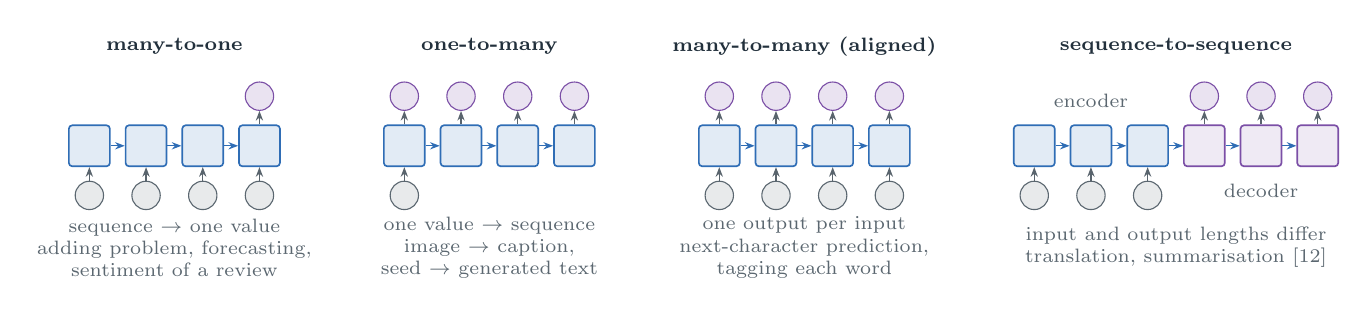
\begin{tikzpicture}[x=7.2mm,y=6.3mm]
  % ---- many-to-one
  \begin{scope}
    \foreach \i in {0,1,2,3} { \node[rc] (c\i) at (\i,0) {}; \node[inp] (x\i) at (\i,-1) {}; \draw[thin flow] (x\i)--(c\i); }
    \foreach \i/\j in {0/1,1/2,2/3} \draw[thin flow,draw=cEmb] (c\i)--(c\j);
    \node[outp] (y) at (3,1) {}; \draw[thin flow] (c3)--(y);
    \node[font=\scriptsize\bfseries,text=cInk] at (1.5,2.0) {many-to-one};
    \node[note] at (1.5,-2.05) {sequence $\to$ one value\\adding problem, forecasting,\\sentiment of a review};
  \end{scope}
  % ---- one-to-many
  \begin{scope}[xshift=40mm]
    \foreach \i in {0,1,2,3} { \node[rc] (c\i) at (\i,0) {}; \node[outp] (y\i) at (\i,1) {}; \draw[thin flow] (c\i)--(y\i); }
    \foreach \i/\j in {0/1,1/2,2/3} \draw[thin flow,draw=cEmb] (c\i)--(c\j);
    \node[inp] (x) at (0,-1) {}; \draw[thin flow] (x)--(c0);
    \node[font=\scriptsize\bfseries,text=cInk] at (1.5,2.0) {one-to-many};
    \node[note] at (1.5,-2.05) {one value $\to$ sequence\\image $\to$ caption,\\seed $\to$ generated text};
  \end{scope}
  % ---- many-to-many
  \begin{scope}[xshift=80mm]
    \foreach \i in {0,1,2,3} { \node[rc] (c\i) at (\i,0) {}; \node[inp] (x\i) at (\i,-1) {}; \node[outp] (y\i) at (\i,1) {};
      \draw[thin flow] (x\i)--(c\i); \draw[thin flow] (c\i)--(y\i); }
    \foreach \i/\j in {0/1,1/2,2/3} \draw[thin flow,draw=cEmb] (c\i)--(c\j);
    \node[font=\scriptsize\bfseries,text=cInk] at (1.5,2.0) {many-to-many (aligned)};
    \node[note] at (1.5,-2.05) {one output per input\\next-character prediction,\\tagging each word};
  \end{scope}
  % ---- sequence-to-sequence
  \begin{scope}[xshift=120mm]
    \foreach \i in {0,1,2} { \node[rc] (c\i) at (\i,0) {}; \node[inp] (x\i) at (\i,-1) {}; \draw[thin flow] (x\i)--(c\i); }
    \foreach \i in {3,4,5} { \node[rc,draw=cOut,fill=cOut!12] (c\i) at (\i,0) {}; \node[outp] (y\i) at (\i,1) {}; \draw[thin flow] (c\i)--(y\i); }
    \foreach \i/\j in {0/1,1/2,2/3,3/4,4/5} \draw[thin flow,draw=cEmb] (c\i)--(c\j);
    \node[font=\scriptsize\bfseries,text=cInk] at (2.5,2.0) {sequence-to-sequence};
    \node[note] at (1,0.9) {encoder}; \node[note] at (4,-0.9) {decoder};
    \node[note] at (2.5,-2.05) {input and output lengths differ\\translation, summarisation \cite{12}};
  \end{scope}
\end{tikzpicture}


\vspace{-1mm}
{\scriptsize\color{cTok}Grey: inputs $x_t$. Blue: the recurrent cell and its state. Purple: outputs.
The same cell is drawn once per time step.\par}
\end{frame}

% ======================================================================= 3
\begin{frame}{Preparing sequence data: windows, ids, and a split by time}
\begin{columns}[T,onlytextwidth]
\column{0.50\textwidth}
\centering
\begin{tikzpicture}
\begin{axis}[width=9.0cm,height=3.55cm,xmin=1749,xmax=1984,ymin=0,ymax=270,axis lines=left,
  tick label style={font=\tiny},xtick={1750,1800,1850,1900,1950},ytick={0,100,200},
  x tick label style={/pgf/number format/1000 sep=},ylabel={sunspots},label style={font=\scriptsize},
  ylabel shift=-3pt,clip=false]
  \fill[cEmb!12] (axis cs:1749,0) rectangle (axis cs:\sunTrainEndYear,255);
  \fill[cAtt!18] (axis cs:\sunTrainEndYear,0) rectangle (axis cs:\sunValEndYear,255);
  \fill[cOut!16] (axis cs:\sunValEndYear,0) rectangle (axis cs:1984,255);
  \addplot[cInk,line width=0.35pt,no marks] table[x=year,y=value]{generated/sunspots.dat};
  \node[font=\scriptsize,text=cEmb!80!black] at (axis cs:1830,238) {train: first 70\% (\sunNtrain{} months)};
  \node[font=\scriptsize,text=cAtt!80!black] at (axis cs:1931,238) {val 15\%};
  \node[font=\scriptsize,text=cOut!80!black] at (axis cs:1967,285) {test 15\%};
\end{axis}
\end{tikzpicture}

\vspace{-0.5mm}
\raggedright\footnotesize
\key{Split by time, never at random.} Neighbouring windows share 23 of their 24 values: a random
split puts near-copies of every test window into training and lets the model learn from the future.

\vspace{1mm}
\centering
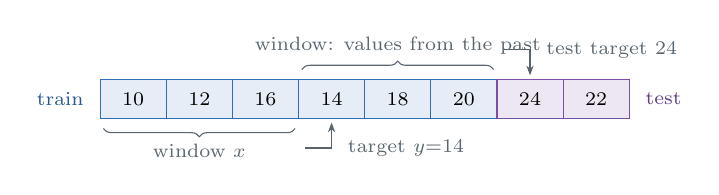
\begin{tikzpicture}[x=8.4mm,y=5mm,font=\scriptsize]
  \foreach \v/\i in {10/0,12/1,16/2,14/3,18/4,20/5}
    \node[draw=cEmb,fill=cEmb!12,minimum width=8.4mm,minimum height=5mm,inner sep=0] at (\i,0) {\v};
  \foreach \v/\i in {24/6,22/7}
    \node[draw=cOut,fill=cOut!14,minimum width=8.4mm,minimum height=5mm,inner sep=0] at (\i,0) {\v};
  \draw[decorate,decoration={brace,amplitude=3pt,mirror},cTok] (-0.45,-0.75)--(2.45,-0.75) node[midway,below=2pt,note]{window $x$};
  \draw[thin flow] (2.6,-1.25) -- (3,-1.25) -- (3,-0.6); \node[note,anchor=west] at (3.1,-1.25) {target $y{=}14$};
  \draw[decorate,decoration={brace,amplitude=3pt},cTok] (2.55,0.75)--(5.45,0.75) node[midway,above=2pt,note]{window: values from the past};
  \draw[thin flow] (5.6,1.25) -- (6,1.25) -- (6,0.6); \node[note,anchor=west] at (6.1,1.25) {test target $24$};
  \node[note,anchor=east,text=cEmb!80!black] at (-0.6,0) {train}; \node[note,anchor=west,text=cOut!80!black] at (7.6,0) {test};
\end{tikzpicture}

\vspace{0.5mm}
\raggedright\footnotesize
\key{Scale with training statistics only}: $\mu=15$, $\sigma=3.42$ from the six training values, so
$16\to(16-15)/3.42=\num{0.293}$. Using all eight values gives $\mu=17$, $\sigma=4.58$: the test period has
leaked. Sunspots: $\mu=\sunMean$, $\sigma=\sunStd$ from 1749--\sunTrainEnd.
\column{0.47\textwidth}
\small
\textbf{Text}: characters (or word pieces) $\to$ integer ids $\to$ vectors.

\vspace{1mm}
\centering
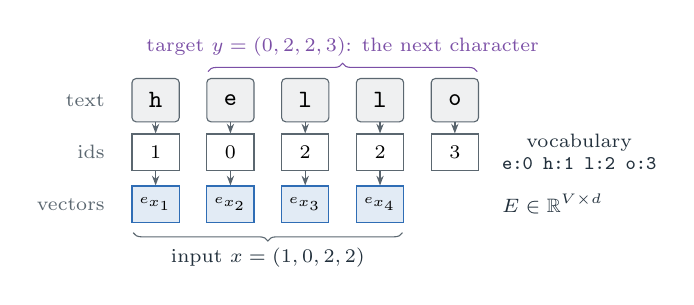
\begin{tikzpicture}[x=9.5mm,y=6.6mm,font=\scriptsize]
  \foreach \ch/\id/\i in {h/1/0,e/0/1,l/2/2,l/2/3,o/3/4} {
    \node[tokbox,minimum width=6mm] (t\i) at (\i,2) {\ch};
    \node[draw=cTok,fill=white,minimum width=6mm,minimum height=4.6mm,inner sep=0] (i\i) at (\i,1) {\id};
    \draw[thin flow] (t\i)--(i\i);
  }
  \foreach \i in {0,1,2,3} {
    \node[draw=cEmb,fill=cEmb!14,minimum width=6mm,minimum height=4.6mm,inner sep=0,font=\tiny] (e\i) at (\i,0) {$e_{x_{\the\numexpr\i+1}}$};
    \draw[thin flow] (i\i)--(e\i);
  }
  \node[note,anchor=east] at (-0.55,2) {text}; \node[note,anchor=east] at (-0.55,1) {ids}; \node[note,anchor=east] at (-0.55,0) {vectors};
  \node[note,anchor=west,text=cInk] at (4.5,1) {vocabulary\\\texttt{e:0 h:1 l:2 o:3}};
  \node[note,anchor=west,text=cInk] at (4.5,0) {$E\in\R^{V\times d}$};
  \draw[decorate,decoration={brace,amplitude=3pt,mirror},cTok] (-0.3,-0.55)--(3.3,-0.55) node[midway,below=2pt,note,text=cInk]{input $x=(1,0,2,2)$};
  \draw[decorate,decoration={brace,amplitude=3pt},cOut] (0.7,2.55)--(4.3,2.55) node[midway,above=2pt,note,text=cOut]{target $y=(0,2,2,3)$: the next character};
\end{tikzpicture}

\vspace{1mm}
\raggedright\footnotesize
\begin{itemize}
  \item \key{One-hot}: id $k$ becomes a vector of $V$ zeros with a 1 at position $k$.
  \item \key{Embedding}: id $k$ selects row $k$ of a learned table $E$: the same as one-hot times a
        weight matrix, without the wasted multiplications. Here $V=\shkVocab$, $d=32$.
  \item The target is the input shifted by one position.\vspace{-1mm}
\end{itemize}
\begin{block}{Checklist (\texttt{data.py})}
\footnotesize
Split first, by position in time; then fit scalers on the training part. A test window may
\emph{read} earlier months (the past is known when forecasting); its \emph{target} must lie in
the test period.
\end{block}
\end{columns}
\end{frame}

% ======================================================================= 4
\begin{frame}{The simple recurrent network (Elman RNN)}
\begin{columns}[T,onlytextwidth]
\column{0.50\textwidth}
\centering
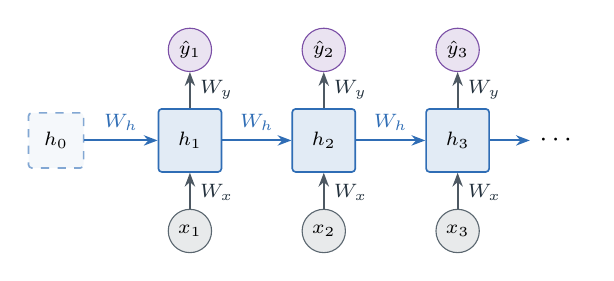
\begin{tikzpicture}[x=17mm,y=10mm]
  \node[rc,minimum size=7mm,fill=cEmb!5,draw=cEmb!60,dashed] (h0) at (0,0) {$h_0$};
  \foreach \i in {1,2,3} {
    \node[rc,minimum size=8mm] (h\i) at (\i,0) {$h_\i$};
    \node[inp,minimum size=5.5mm,font=\scriptsize] (x\i) at (\i,-1.15) {$x_\i$};
    \node[outp,minimum size=5.5mm,font=\scriptsize] (y\i) at (\i,1.15) {$\hat y_\i$};
    \draw[flow] (x\i)-- node[right,note,text=cInk,pos=0.45]{$W_x$} (h\i);
    \draw[flow] (h\i)-- node[right,note,text=cInk,pos=0.5]{$W_y$} (y\i);
  }
  \foreach \i/\j in {0/1,1/2,2/3} \draw[flow,draw=cEmb] (h\i)-- node[above,note,text=cEmb]{$W_h$} (h\j);
  \node (dots) at (3.75,0) {$\cdots$}; \draw[flow,draw=cEmb] (h3)--(dots);
\end{tikzpicture}
\vspace{-1mm}
\begin{block}{One rule, applied at every step $t=1,\dots,T$}
\vspace{-2.5mm}
\[
  h_t=\tanh\bigl(W_x\,x_t+W_h\,h_{t-1}+b\bigr),\qquad \hat y_t=W_y\,h_t+b_y
\]
\vspace{-4mm}

{\footnotesize $x_t\in\R^{n_\text{in}}$, \ $h_t\in\R^{n_h}$, \ $W_x\in\R^{n_h\times n_\text{in}}$, \
$W_h\in\R^{n_h\times n_h}$, \ $h_0=0$.}
\end{block}
\footnotesize\raggedright
\begin{itemize}
  \item The \key{hidden state} $h_t$ is the network's only memory: everything it knows about
        $x_1..x_t$ must fit in $n_h$ numbers.
  \item \key{Unrolling}: drawn over time, the RNN is a deep network with one layer per time step.
  \item \key{Parameter sharing}: every step uses the same $W_x,W_h,b$. The count,
        $(n_\text{in}+n_h+1)\,n_h$, does not depend on $T$; a pattern learned at one position
        works at all positions \cite{1}.
\end{itemize}
\column{0.47\textwidth}
\small
\textbf{Two steps by hand} \ ($n_\text{in}=1$, $n_h=2$, $h_0=0$)
{\footnotesize
\[
 W_x=\begin{bmatrix}0.5\\-1\end{bmatrix},\quad
 W_h=\begin{bmatrix}0.5&-0.5\\0.25&1\end{bmatrix},\quad
 b=\begin{bmatrix}0\\0.5\end{bmatrix}
\]
\vspace{-2mm}
\renewcommand{\arraystretch}{1.15}
\begin{tabular}{@{}l@{\ \ }l@{}}
$x_1=1$: & $z_1=W_x\cdot1+W_h h_0+b=(0.5,\,-0.5)$\\
 & $h_1=\tanh z_1=(\num{0.462},\,\num{-0.462})$\\
$x_2=2$: & $z_2=W_x\cdot2+W_h h_1+b$\\
 & $\phantom{z_2}=(1,-2)+(0.462,-0.347)+(0,0.5)$\\
 & $\phantom{z_2}=(1.462,\,-1.847)$\\
 & $h_2=\tanh z_2=(\num{0.898},\,\num{-0.951})$
\end{tabular}}

\vspace{1mm}
\begin{block}{What to notice}
\footnotesize
\begin{itemize}
  \item $h_2$ depends on $x_1$ only through $h_1$: the past reaches the present through the state
        and nothing else.
  \item $\tanh$ keeps every state in $(-1,1)$: the state cannot blow up.
  \item 8 parameters here: $(1+2+1)\cdot2$. A sequence of 2 steps or 2{,}000 uses the same 8.
  \item The output layer $W_y$ is an ordinary linear layer, used at every step
        (many-to-many) or only at $t=T$ (many-to-one).
\end{itemize}
\end{block}
{\scriptsize\color{cTok}\texttt{walkthrough.py}, section 3, prints these numbers.\par}
\end{columns}
\end{frame}

% ======================================================================= 5
\begin{frame}{Backpropagation through time and the product of Jacobians}
\begin{columns}[T,onlytextwidth]
\column{0.50\textwidth}
\centering
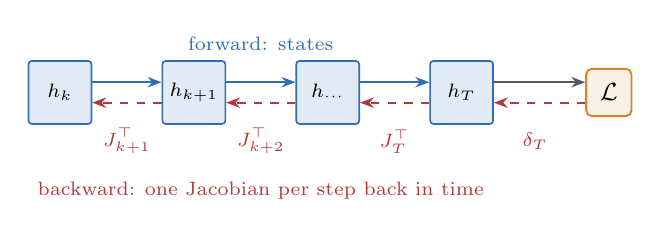
\begin{tikzpicture}[x=17mm,y=10mm]
  \foreach \i/\l in {1/k,2/k{+}1,3/\cdots,4/T} {
    \node[rc,minimum size=8mm] (h\i) at (\i,0) {$h_{\l}$};
  }
  \foreach \i/\j in {1/2,2/3,3/4} {
    \draw[flow,draw=cEmb] ([yshift=1.3mm]h\i.east)--([yshift=1.3mm]h\j.west);
    \draw[flow,draw=cBad,dashed] ([yshift=-1.3mm]h\j.west)--([yshift=-1.3mm]h\i.east);
  }
  \node[stage=cAtt,minimum height=6mm] (L) at (5.1,0) {$\mathcal L$};
  \draw[flow] ([yshift=1.3mm]h4.east)--([yshift=1.3mm]L.west);
  \draw[flow,draw=cBad,dashed] ([yshift=-1.3mm]L.west)--([yshift=-1.3mm]h4.east);
  \node[note,text=cBad] at (1.5,-0.62) {$J_{k+1}^{\T}$}; \node[note,text=cBad] at (2.5,-0.62) {$J_{k+2}^{\T}$};
  \node[note,text=cBad] at (3.5,-0.62) {$J_{T}^{\T}$}; \node[note,text=cBad] at (4.55,-0.62) {$\delta_T$};
  \node[note,text=cEmb] at (2.5,0.62) {forward: states};
  \node[note,text=cBad] at (2.5,-1.25) {backward: one Jacobian per step back in time};
\end{tikzpicture}

\vspace{0.5mm}
\raggedright\small
Unrolled, the RNN is a deep network and the chain rule applies: \key{backpropagation through
time} (BPTT) \cite{2}. Let $\delta_t=\partial\mathcal L/\partial h_t$, with the loss at the last step.
\begin{block}{One step back multiplies by one Jacobian}
\vspace{-3mm}
\begin{gather*}
  J_t=\frac{\partial h_t}{\partial h_{t-1}}=\diag\!\bigl(1-h_t^{2}\bigr)\,W_h,
  \qquad\delta_{t-1}=J_t^{\T}\,\delta_t\\[1pt]
  \delta_k=\bigl(J_T\,J_{T-1}\cdots J_{k+1}\bigr)^{\T}\delta_T\\[1pt]
  \frac{\partial\mathcal L}{\partial W_h}=\sum_{t=1}^{T}\bigl(\delta_t\odot(1-h_t^2)\bigr)\,h_{t-1}^{\T}
\end{gather*}
\vspace{-4.5mm}
\end{block}
{\footnotesize Shared weights: the gradient is a \emph{sum over time steps}; the term linking
step $k$ to the loss carries a product of $T-k$ Jacobians.}
\column{0.47\textwidth}
\small
\textbf{A product of many similar factors either shrinks or grows.} With
$\sigma_{\max}$ the largest singular value of $W_h$ and $\tanh'\le1$:
\[
  \|\delta_k\|\;\le\;\bigl(\sigma_{\max}(W_h)\bigr)^{T-k}\,\|\delta_T\|
\]
\vspace{-4mm}
\begin{itemize}\footnotesize
  \item \key{Vanishing} ($\sigma_{\max}<1$, or saturated $\tanh$): the signal from $T-k$ steps back
        decays exponentially. $0.9^{50}=0.005$, $0.9^{100}=3\times10^{-5}$. The total gradient is
        not zero; it is dominated by the recent past, so \textbf{long-range dependencies are not
        learned} \cite{3}.
  \item \key{Exploding} (needs $\sigma_{\max}>1$): $1.1^{50}=117$, $1.1^{100}=1.4\times10^{4}$. One
        huge step can wreck the weights. Remedy: clipping (slide 12) \cite{4}.
\end{itemize}
\begin{block}{The core difficulty}
\footnotesize
To store information reliably the state must be stable under small perturbations, which
means $\|J_t\|<1$: exactly the condition for vanishing gradients \cite{3}. Tuning $W_h$ cannot
fix this. The architecture must change (slides 6--9).
\end{block}
\end{columns}
\end{frame}

% ======================================================================= 6
\begin{frame}{The LSTM cell: three gates and a separate memory}
\begin{columns}[T,onlytextwidth]
\column{0.57\textwidth}
\centering
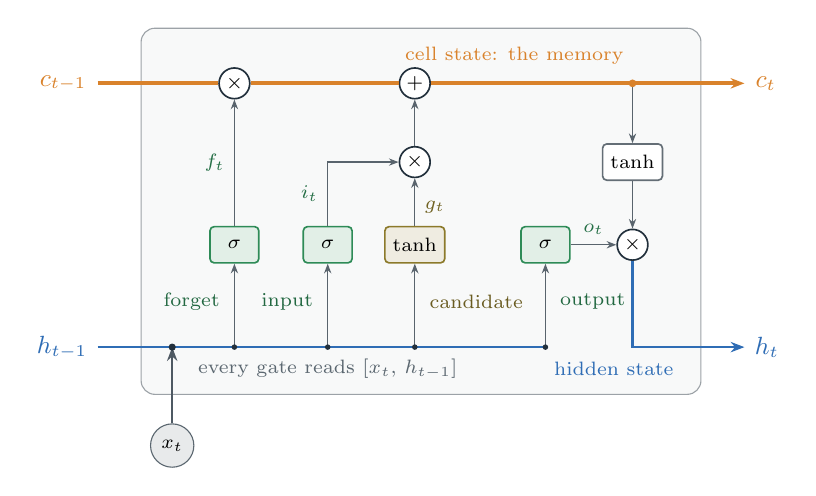
\begin{tikzpicture}[x=7.9mm,y=10mm]
  % cell boundary
  \begin{scope}[on background layer]
    \draw[draw=cInk!45,fill=cInk!3,rounded corners=5pt] (0,0.1) rectangle (9.0,4.75);
  \end{scope}
  % cell-state line
  \node[op] (mf) at (1.5,4.05) {$\times$};
  \node[op] (add) at (4.4,4.05) {$+$};
  \draw[cline] (-0.7,4.05) node[left,text=cAtt,font=\small]{$c_{t-1}$} -- (mf);
  \draw[cline] (mf)--(add);
  \draw[cline,->] (add)--(9.7,4.05) node[right,text=cAtt,font=\small]{$c_t$};
  % bottom bus: h_{t-1} and x_t
  \draw[line width=0.9pt,draw=cEmb] (-0.7,0.7) node[left,text=cEmb,font=\small]{$h_{t-1}$} -- (6.5,0.7);
  \node[inp,minimum size=5.5mm,font=\scriptsize] (x) at (0.5,-0.55) {$x_t$};
  \draw[flow] (x)--(0.5,0.7);
  \fill[cInk] (0.5,0.7) circle (1.3pt);
  % gates
  \node[gate] (f) at (1.5,2.0) {$\sig$};
  \node[gate] (i) at (3.0,2.0) {$\sig$};
  \node[cand] (g) at (4.4,2.0) {$\tanh$};
  \node[gate] (o) at (6.5,2.0) {$\sig$};
  \foreach \n/\xx in {f/1.5,i/3.0,g/4.4,o/6.5} { \draw[thin flow] (\xx,0.7)--(\n); \fill[cInk] (\xx,0.7) circle (1pt); }
  \node[op] (mi) at (4.4,3.05) {$\times$};
  \draw[thin flow] (f)-- node[left,font=\scriptsize,text=cFfn!80!black]{$f_t$} (mf);
  \draw[thin flow] (i) |- node[pos=0.25,left,font=\scriptsize,text=cFfn!80!black]{$i_t$} (mi);
  \draw[thin flow] (g)-- node[right,font=\scriptsize,text=cNrm!80!black,pos=0.4]{$g_t$} (mi);
  \draw[thin flow] (mi)--(add);
  % output side
  \node[cand,draw=cInk!70,fill=white] (tc) at (7.9,3.05) {$\tanh$};
  \node[op] (mo) at (7.9,2.0) {$\times$};
  \draw[thin flow] (7.9,4.05)--(tc); \fill[cAtt] (7.9,4.05) circle (1.4pt);
  \draw[thin flow] (tc)--(mo);
  \draw[thin flow] (o)-- node[above,font=\scriptsize,text=cFfn!80!black]{$o_t$} (mo);
  \draw[line width=0.9pt,draw=cEmb,->] (mo) |- (9.7,0.7) node[right,text=cEmb,font=\small]{$h_t$};
  % labels
  \node[note,text=cFfn!75!black,anchor=east] at (1.42,1.28) {forget}; \node[note,text=cFfn!75!black,anchor=east] at (2.92,1.28) {input};
  \node[note,text=cNrm!75!black,anchor=west] at (4.48,1.28) {candidate}; \node[note,text=cFfn!75!black,anchor=west] at (6.58,1.28) {output};
  \node[note,text=cAtt] at (6.0,4.4) {cell state: the memory};
  \node[note,text=cEmb] at (7.6,0.42) {hidden state};
  \node[note] at (3.0,0.42) {every gate reads $[x_t,\,h_{t-1}]$};
\end{tikzpicture}

\vspace{0.5mm}
\raggedright\footnotesize
\begin{itemize}
  \item A \key{gate} is a sigmoid layer whose outputs in $(0,1)$ multiply another vector
        elementwise: 0 blocks a component, 1 lets it through.
  \item Two states: the \key{cell state} $c_t$ stores, the hidden state $h_t$ is what the gates,
        the next layer and the output see.
  \item The 1997 LSTM \cite{5} had input and output gates; the forget gate was added in 2000 \cite{6}.
\end{itemize}
\column{0.41\textwidth}
\small
\begin{block}{The six equations}
\vspace{-3.5mm}
\begin{align*}
 f_t&=\sig\bigl(W_f\,[x_t,h_{t-1}]+b_f\bigr) && \text{\scriptsize forget}\\
 i_t&=\sig\bigl(W_i\,[x_t,h_{t-1}]+b_i\bigr) && \text{\scriptsize input}\\
 g_t&=\tanh\bigl(W_g\,[x_t,h_{t-1}]+b_g\bigr) && \text{\scriptsize candidate}\\
 o_t&=\sig\bigl(W_o\,[x_t,h_{t-1}]+b_o\bigr) && \text{\scriptsize output}\\[2pt]
 c_t&=f_t\odot c_{t-1}+i_t\odot g_t && \text{\scriptsize cell}\\
 h_t&=o_t\odot\tanh(c_t) && \text{\scriptsize hidden}
\end{align*}
\vspace{-5mm}
\end{block}
\footnotesize
$[x_t,h_{t-1}]\in\R^{n_\text{in}+n_h}$ is the two vectors stacked; $\sig(z)=1/(1+e^{-z})$;
$\odot$ is the elementwise product.

\vspace{1mm}
\textbf{Read the cell update as a sentence}: keep a fraction $f_t$ of the old memory, and add a
fraction $i_t$ of the new candidate $g_t$.

\vspace{1mm}
\textbf{In one line}: stack the four weight matrices into $W\in\R^{4n_h\times(n_\text{in}+n_h)}$,
compute $z_t=W[x_t,h_{t-1}]+b$ once and split it in four. That is what the code does (slide 15).
\end{columns}
\end{frame}

% ======================================================================= 7
\begin{frame}{One LSTM step by hand}
\begin{columns}[T,onlytextwidth]
\column{0.52\textwidth}
\small
Smallest possible cell: $n_\text{in}=1$, $n_h=1$. Inputs to this step:
\[
  x_t=1,\qquad h_{t-1}=0.5,\qquad c_{t-1}=1.0
\]
\vspace{-4mm}

{\footnotesize
\renewcommand{\arraystretch}{1.25}
\begin{tabular}{@{}l@{\ \ }r@{\ \ }r@{\ \ }r@{\quad}l@{\ }l@{}}
\toprule
 & $w_x$ & $w_h$ & $b$ & $z=w_x x_t+w_h h_{t-1}+b$ & value\\
\midrule
forget $f$ & $0.5$ & $1$ & $1$ & $0.5+0.5+1=2$ & $\sig(2)=\num{0.881}$\\
input $i$ & $1$ & $-2$ & $0$ & $1-1+0=0$ & $\sig(0)=\num{0.500}$\\
candidate $g$ & $0.5$ & $1$ & $0$ & $0.5+0.5+0=1$ & $\tanh(1)=\num{0.762}$\\
output $o$ & $1$ & $2$ & $-1$ & $1+1-1=1$ & $\sig(1)=\num{0.731}$\\
\bottomrule
\end{tabular}}

\vspace{1mm}
{\footnotesize
\begin{align*}
  c_t&=f\,c_{t-1}+i\,g=0.881\cdot1.0+0.500\cdot0.762=0.881+0.381=\num{1.262}\\
  h_t&=o\,\tanh(c_t)=0.731\cdot\tanh(1.262)=0.731\cdot0.852=\num{0.623}
\end{align*}}
\vspace{-4mm}

\centering
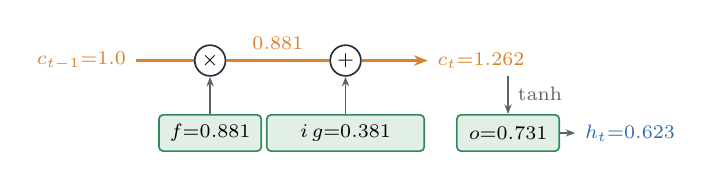
\begin{tikzpicture}[x=8.6mm,y=8mm,font=\scriptsize]
  \node[text=cAtt] (c0) at (0,0) {$c_{t-1}{=}1.0$};
  \node[op] (m) at (1.9,0) {$\times$}; \node[op] (a) at (3.9,0) {$+$};
  \node[text=cAtt] (c1) at (5.9,0) {$c_t{=}1.262$};
  \draw[cline] (c0)--(m); \draw[cline] (m)-- node[above,text=cAtt]{$0.881$} (a); \draw[cline,->] (a)--(c1);
  \node[gate,minimum width=13mm] (f) at (1.9,-1.15) {$f{=}0.881$};
  \node[gate,minimum width=20mm] (ig) at (3.9,-1.15) {$i\,g{=}0.381$};
  \draw[thin flow] (f)--(m); \draw[thin flow] (ig)--(a);
  \node[gate,minimum width=13mm] (o) at (6.3,-1.15) {$o{=}0.731$};
  \node[text=cEmb] (h) at (8.1,-1.15) {$h_t{=}0.623$};
  \draw[thin flow] (6.3,-0.25) -- node[right,note,pos=0.45]{$\tanh$} (o.north); \draw[thin flow] (o)--(h);
\end{tikzpicture}
\column{0.45\textwidth}
\small
\begin{block}{Reading the numbers}
\footnotesize
\begin{itemize}
  \item \textbf{Forget gate 0.88}: 88\% of the old memory survives. The bias $b_f=1$ contributes half
        of $z_f$; without it $f=\sig(1)=0.73$.
  \item \textbf{Input gate 0.5} lets half of the candidate $0.762$ in.
  \item The cell state \emph{grew} above 1. It is not squashed, so it can count and accumulate.
  \item \textbf{Output gate 0.73}: $h_t$ is a squashed, scaled view of the memory.
        A cell can hold a value while $o\approx0$ hides it.
\end{itemize}
\end{block}
\footnotesize
\textbf{Next step with $x_{t+1}=0$}: $c_{t+1}=1.177$, $h_{t+1}=0.464$. The memory fades slowly at a
rate set by $f$, not by a weight matrix.

\vspace{1.5mm}
\textbf{The local derivative that matters}: along the cell state,
$\partial c_t/\partial c_{t-1}=f_t=0.881$ on the direct path. In an RNN the corresponding factor is
$\partial h_t/\partial h_{t-1}=(1-h_t^2)\,w_h$.

\vspace{1mm}
\textbf{Parameters}: 4 rows of $(w_x,w_h,b)$ = $4\,(1+1+1)\cdot1=12$.

\vspace{1.5mm}
{\scriptsize\color{cTok}\texttt{walkthrough.py}, section 5, prints every number here and checks it
against \texttt{lstm\_numpy.lstm\_step} and \texttt{lstm.LSTMCellScratch}.\par}
\end{columns}
\end{frame}

% ======================================================================= 8
\begin{frame}{Why it works: the cell state is a conveyor belt}
\begin{columns}[T,onlytextwidth]
\column{0.52\textwidth}
\centering
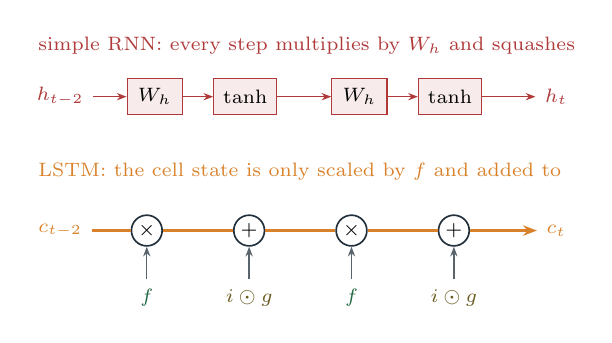
\begin{tikzpicture}[x=10mm,y=10mm,font=\scriptsize]
  % RNN chain
  \node[note,anchor=west,text=cBad] at (-0.6,1.05) {simple RNN: every step multiplies by $W_h$ and squashes};
  \node[text=cBad] (r0) at (-0.2,0.4) {$h_{t-2}$};
  \foreach \k/\xx in {1/1.0,2/3.6} {
    \node[draw=cBad,fill=cBad!10,minimum width=7mm,minimum height=4.6mm,inner sep=0] (w\k) at (\xx,0.4) {$W_h$};
    \node[draw=cBad,fill=cBad!10,minimum width=8mm,minimum height=4.6mm,inner sep=0] (t\k) at (\xx+1.15,0.4) {$\tanh$};
    \draw[thin flow,draw=cBad] (w\k)--(t\k);
  }
  \node[text=cBad] (r2) at (6.1,0.4) {$h_{t}$};
  \draw[thin flow,draw=cBad] (r0)--(w1); \draw[thin flow,draw=cBad] (t1)--(w2); \draw[thin flow,draw=cBad] (t2)--(r2);
  % LSTM belt
  \node[note,anchor=west,text=cAtt] at (-0.6,-0.55) {LSTM: the cell state is only scaled by $f$ and added to};
  \node[text=cAtt] (c0) at (-0.2,-1.3) {$c_{t-2}$};
  \foreach \k/\xx in {1/0.9,2/3.5} {
    \node[op] (m\k) at (\xx,-1.3) {$\times$}; \node[op] (a\k) at (\xx+1.3,-1.3) {$+$};
    \draw[cline] (m\k)--(a\k);
    \node[text=cFfn!75!black] (f\k) at (\xx,-2.15) {$f$}; \node[text=cNrm!75!black] (g\k) at (\xx+1.3,-2.15) {$i\odot g$};
    \draw[thin flow] (f\k)--(m\k); \draw[thin flow] (g\k)--(a\k);
  }
  \node[text=cAtt] (c2) at (6.1,-1.3) {$c_{t}$};
  \draw[cline] (c0)--(m1); \draw[cline] (a1)--(m2); \draw[cline,->] (a2)--(c2);
\end{tikzpicture}

\vspace{0.5mm}
\raggedright\small
Differentiate $c_t=f_t\odot c_{t-1}+i_t\odot g_t$ along the belt:
\begin{block}{The direct path has no weight matrix and no squashing}
\vspace{-3mm}
\[
  \frac{\partial c_t}{\partial c_{t-1}}=\diag(f_t)+\bigl(\text{terms via }h_{t-1}\bigr),
  \;\;
  \frac{\partial c_T}{\partial c_k}\Big|_{\text{direct}}=\diag\Bigl(\prod_{t=k+1}^{T}\!f_t\Bigr)
\]
\vspace{-4mm}
\end{block}
{\footnotesize With $f_t=1$ and $i_t=0$ the cell copies itself and the gradient passes back
unchanged: the \key{constant error carousel} of \cite{5}. Residual connections in deep networks
rely on the same additive idea.}
\column{0.45\textwidth}
\small
\textbf{The decay rate is now learned}, per unit and per step:

\vspace{1mm}
{\footnotesize
\renewcommand{\arraystretch}{1.2}
\begin{tabular}{@{}lccc@{}}
\toprule
forget gate $f$ & $f^{20}$ & $f^{50}$ & $f^{100}$\\
\midrule
$\sig(0)=0.50$ & $10^{-6}$ & $9\times10^{-16}$ & $8\times10^{-31}$\\
$\sig(1)=0.73$ & $0.002$ & $2\times10^{-7}$ & $2\times10^{-14}$\\
$0.99$ & $0.82$ & $0.61$ & $0.37$\\
\bottomrule
\end{tabular}}

\vspace{1.5mm}
\begin{block}{Why the forget-gate bias starts at 1}
\footnotesize
With all biases 0 a fresh LSTM has $f\approx0.5$: it forgets half its memory every step and
gradients vanish as fast as in an RNN (slide 9). Setting $b_f=1$ starts the gates mostly
open \cite{6,8}. Keras does this by default; PyTorch does not (\texttt{set\_forget\_bias} in
\texttt{lstm.py}).

\vspace{1mm}
Measured, adding problem, $T=40$, steps until validation MSE $<0.01$ for \addSeeds{} seeds.
$b_f=0$: \fbZeroSteps. \ $b_f=1$: \fbOneSteps. A modest gain at this length.
\end{block}
{\footnotesize \textbf{Not solved}: $h_t$ still feeds the gates through weight matrices, where
gradients can explode, so clipping stays (slide 12).}
\end{columns}
\end{frame}

% ======================================================================= 9
\begin{frame}{Measured: how far back does the gradient reach?}
\begin{columns}[T,onlytextwidth]
\column{0.56\textwidth}
\centering
\begin{tikzpicture}
\begin{semilogyaxis}[width=9.6cm,height=5.7cm,xmin=0,xmax=100,ymin=1e-16,ymax=30,
  xlabel={steps back in time, $T-t$},ylabel={$\|\partial\mathcal L/\partial\,\text{state}_t\|$ relative to $t=T$},
  label style={font=\scriptsize},tick label style={font=\tiny},axis lines=left,ymajorgrids,grid style={cInk!10},
  ytick={1e-15,1e-12,1e-9,1e-6,1e-3,1},
  legend columns=2,legend style={font=\scriptsize,draw=none,fill=none,at={(0.46,-0.2)},anchor=north,/tikz/every even column/.append style={column sep=3mm}},legend cell align=left,
  every axis plot/.append style={line width=1.2pt,no marks}]
  \addplot[cAtt] table[x=lag,y=lstmtrained]{generated/gradlag.dat}; \addlegendentry{LSTM, trained (adding problem)}
  \addplot[cAtt,dashed] table[x=lag,y=lstmone]{generated/gradlag.dat}; \addlegendentry{LSTM at initialisation, $b_f=1$}
  \addplot[cAtt,densely dotted] table[x=lag,y=lstmzero]{generated/gradlag.dat}; \addlegendentry{LSTM at initialisation, $b_f=0$}
  \addplot[cBad] table[x=lag,y=rnn]{generated/gradlag.dat}; \addlegendentry{simple RNN at initialisation}
\end{semilogyaxis}
\end{tikzpicture}

\vspace{-0.5mm}
\raggedright
{\scriptsize\color{cTok}Measured by \texttt{experiments.py grad}: $n_h=32$, sequences of length 100 from the adding
problem, loss at the last step only. State = $h_t$ (RNN) or $(h_t,c_t)$ (LSTM). Initialisation curves:
geometric mean of 5 seeds, PyTorch default weights. Trained curve: one model.\par}
\column{0.41\textwidth}
\small
{\footnotesize
\renewcommand{\arraystretch}{1.25}
\begin{tabular}{@{}lcc@{}}
\toprule
gradient norm ratio & 20 back & 50 back\\
\midrule
RNN, init & $\gradRnnTwenty$ & $\gradRnnFifty$\\
LSTM, init, $b_f=0$ & $\gradLstmzeroTwenty$ & $\gradLstmzeroFifty$\\
LSTM, init, $b_f=1$ & $\gradLstmoneTwenty$ & $\gradLstmoneFifty$\\
LSTM, trained & $\gradLstmtrainedTwenty$ & $\gradLstmtrainedFifty$\\
\bottomrule
\end{tabular}}

\vspace{1.5mm}
\begin{itemize}\footnotesize
  \item \textbf{RNN}: a straight line on a log axis is exponential decay, as slide 5
        predicts.
  \item \textbf{An untrained LSTM also vanishes.} With $b_f=0$ it is no better than the RNN.
        The architecture \emph{permits} long memory; it does not guarantee it.
  \item \textbf{$b_f=1$} slows the decay by many orders of magnitude.
  \item \textbf{After training} (\gradTrainedSteps{} steps, test MSE \gradTrainedMse) the gradient 100
        steps back is still $\gradLstmtrainedEnd$ of its final value. The most open unit
        averages $f=\gradTrainedFmax$; the mean over all units is only \gradTrainedFmean.
\end{itemize}
{\footnotesize Gating gives a \emph{learnable} memory span: units that must remember keep
$f\approx1$, the rest stay free to forget.}
\end{columns}
\end{frame}

% ====================================================================== 10
\begin{frame}{Variants: counting parameters, GRU, stacked and bidirectional}
\begin{columns}[T,onlytextwidth]
\column{0.50\textwidth}
\small
\textbf{Counting.} Each gate or candidate is one layer on $[x_t,h_{t-1}]$.

\vspace{0.5mm}
{\footnotesize
\renewcommand{\arraystretch}{1.15}
\begin{tabular}{@{}llrr@{}}
\toprule
 & formula & $n_\text{in}{=}32,\,n_h{=}256$ & \texttt{torch.nn}\\
\midrule
RNN & $\phantom{4}(n_\text{in}+n_h+1)\,n_h$ & \countRnnBook & \countRnnTorch\\
GRU & $3\,(n_\text{in}+n_h+1)\,n_h$ & \countGruBook & \countGruTorch\\
LSTM & $4\,(n_\text{in}+n_h+1)\,n_h$ & \countLstmBook & \countLstmTorch\\
\bottomrule
\end{tabular}}

\vspace{0.5mm}
{\footnotesize PyTorch keeps two bias vectors per layer (\texttt{bias\_ih}, \texttt{bias\_hh}): $4n_h=1{,}024$
extra for the LSTM. Our \texttt{LSTMCellScratch} has exactly \countScratch.}

\vspace{1mm}
\begin{block}{GRU: two gates, one state \cite{9}}
\vspace{-3.5mm}
\begin{align*}
 z_t&=\sig\bigl(W_z[x_t,h_{t-1}]+b_z\bigr) && \text{\scriptsize update}\\
 r_t&=\sig\bigl(W_r[x_t,h_{t-1}]+b_r\bigr) && \text{\scriptsize reset}\\
 n_t&=\tanh\bigl(W_n[x_t,\;r_t\odot h_{t-1}]+b_n\bigr) && \text{\scriptsize candidate}\\
 h_t&=z_t\odot h_{t-1}+(1-z_t)\odot n_t && \text{\scriptsize state}
\end{align*}
\vspace{-5mm}
\end{block}
{\footnotesize The update gate is forget and input gate in one ($f=z$, $i=1-z$); no separate cell,
no output gate. Neither GRU nor LSTM wins consistently \cite{7,10}.}
\column{0.47\textwidth}
\centering
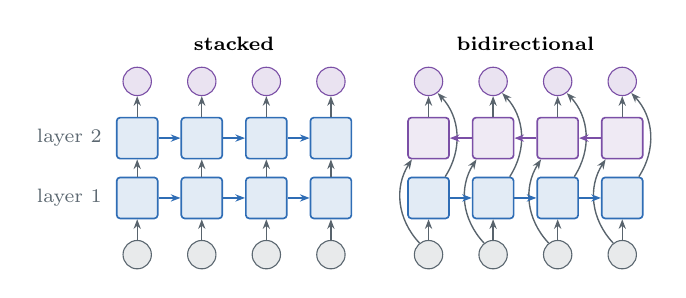
\begin{tikzpicture}[x=8.2mm,y=8mm]
  % stacked
  \begin{scope}
  \foreach \i in {0,1,2,3} {
    \node[inp] (x\i) at (\i,-0.9) {};
    \node[rc] (a\i) at (\i,0) {}; \node[rc] (b\i) at (\i,0.95) {};
    \node[outp] (y\i) at (\i,1.85) {};
    \draw[thin flow] (x\i)--(a\i); \draw[thin flow] (a\i)--(b\i); \draw[thin flow] (b\i)--(y\i);
  }
  \foreach \i/\j in {0/1,1/2,2/3} { \draw[thin flow,draw=cEmb] (a\i)--(a\j); \draw[thin flow,draw=cEmb] (b\i)--(b\j); }
  \node[note,anchor=east] at (-0.4,0) {layer 1}; \node[note,anchor=east] at (-0.4,0.95) {layer 2};
  \node[font=\scriptsize\bfseries] at (1.5,2.45) {stacked};
  \end{scope}
  % bidirectional
  \begin{scope}[xshift=37mm]
  \foreach \i in {0,1,2,3} {
    \node[inp] (x\i) at (\i,-0.9) {};
    \node[rc] (a\i) at (\i,0) {}; \node[rc,draw=cOut,fill=cOut!12] (b\i) at (\i,0.95) {};
    \node[outp] (y\i) at (\i,1.85) {};
    \draw[thin flow] (x\i)--(a\i); \draw[thin flow] (b\i)--(y\i);
    \draw[thin flow] (x\i) to[bend left=38] (b\i); \draw[thin flow] (a\i) to[bend right=38] (y\i);
  }
  \foreach \i/\j in {0/1,1/2,2/3} { \draw[thin flow,draw=cEmb] (a\i)--(a\j); \draw[thin flow,draw=cOut] (b\j)--(b\i); }
  \node[font=\scriptsize\bfseries] at (1.5,2.45) {bidirectional};

  \end{scope}
\end{tikzpicture}

\vspace{1mm}
\raggedright\footnotesize
\begin{itemize}
  \item \key{Stacked}: layer $\ell$ reads the hidden states of layer $\ell-1$ as its input sequence.
        Depth in space on top of depth in time; 2--4 layers were typical \cite{12,15}
        (\texttt{-{}-layers}).
  \item \key{Bidirectional} \cite{11}: a second RNN (purple) reads right to left; the two hidden
        states are concatenated, so each output sees past \emph{and} future. Doubles the
        parameters (\texttt{-{}-bidirectional}).
  \item Bidirectional models suit tagging and classifying complete sequences. They cannot
        forecast or generate: at step $t$ the future does not exist yet.
  \item \key{When GRU?} Smaller models, less data, tight latency budgets. \key{When LSTM?} When a
        separate, unsquashed memory helps: counting, long gaps.
\end{itemize}
\end{columns}
\end{frame}

% ====================================================================== 11
\begin{frame}{Measured: does gating matter? The adding problem}
\begin{columns}[T,onlytextwidth]
\column{0.50\textwidth}
\centering
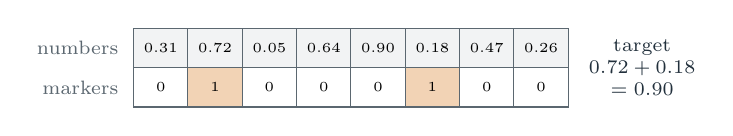
\begin{tikzpicture}[x=6.9mm,y=5mm,font=\scriptsize]
  \foreach \v/\i in {0.31/0,0.72/1,0.05/2,0.64/3,0.90/4,0.18/5,0.47/6,0.26/7}
    \node[draw=cTok,fill=cTok!8,minimum width=6.9mm,minimum height=5mm,inner sep=0,font=\tiny] at (\i,1) {\v};
  \foreach \v/\i/\c in {0/0/white,1/1/cAtt!35,0/2/white,0/3/white,0/4/white,1/5/cAtt!35,0/6/white,0/7/white}
    \node[draw=cTok,fill=\c,minimum width=6.9mm,minimum height=5mm,inner sep=0,font=\tiny] at (\i,0) {\v};
  \node[note,anchor=east] at (-0.6,1) {numbers}; \node[note,anchor=east] at (-0.6,0) {markers};
  \node[note,anchor=west,text=cInk] at (7.7,0.5) {target\\$0.72+0.18$\\$=0.90$};
\end{tikzpicture}

\vspace{1mm}
\begin{tikzpicture}
\begin{semilogyaxis}[width=8.6cm,height=5.5cm,xmin=0,xmax=2000,ymin=0.0003,ymax=0.6,
  xlabel={training step},ylabel={validation MSE, $T=80$},label style={font=\scriptsize},tick label style={font=\tiny},
  axis lines=left,ymajorgrids,grid style={cInk!10},
  legend style={font=\scriptsize,draw=none,fill=none,at={(0.98,0.52)},anchor=east},legend cell align=left,
  every axis plot/.append style={line width=1.2pt,no marks}]
  \addplot[cBad] table[x=step,y=rnn]{generated/adding_curve.dat}; \addlegendentry{simple RNN}
  \addplot[cAtt] table[x=step,y=lstm]{generated/adding_curve.dat}; \addlegendentry{LSTM}
  \addplot[cNrm,dashed] table[x=step,y=gru]{generated/adding_curve.dat}; \addlegendentry{GRU}
  \addplot[cTok,densely dotted,line width=0.8pt,domain=0:2000,samples=2] {\addBaseline};
  \node[font=\tiny,text=cTok,anchor=south west] at (axis cs:1050,0.24) {always predict 1.0: MSE \addBaseline};
\end{semilogyaxis}
\end{tikzpicture}

\vspace{-0.5mm}
{\scriptsize\color{cTok}Seed 0 of each model. A run stops once validation MSE $<0.001$.\par}
\column{0.47\textwidth}
\small
\textbf{The task} \cite{5}: output the sum of the two marked numbers. One marker lies in each
half of the sequence, so the gap is about $T/2$ steps.

\vspace{0.5mm}
{\footnotesize
\renewcommand{\arraystretch}{1.08}
\begin{tabular}{@{}lcccc@{}}
\toprule
solved in $\le2000$ steps & $T{=}10$ & $T{=}20$ & $T{=}40$ & $T{=}80$\\
\midrule
simple RNN & \addRnnSolvedTen/\addSeeds & \addRnnSolvedTwenty/\addSeeds & \addRnnSolvedForty/\addSeeds & \addRnnSolvedEighty/\addSeeds\\
LSTM & \addLstmSolvedTen/\addSeeds & \addLstmSolvedTwenty/\addSeeds & \addLstmSolvedForty/\addSeeds & \addLstmSolvedEighty/\addSeeds\\
GRU & \addGruSolvedTen/\addSeeds & \addGruSolvedTwenty/\addSeeds & \addGruSolvedForty/\addSeeds & \addGruSolvedEighty/\addSeeds\\
\midrule
\multicolumn{5}{@{}l}{median steps until validation MSE $<0.01$}\\
simple RNN & \addRnnStepsTen & \addRnnStepsTwenty & \addRnnStepsForty & \addRnnStepsEighty\\
LSTM & \addLstmStepsTen & \addLstmStepsTwenty & \addLstmStepsForty & \addLstmStepsEighty\\
GRU & \addGruStepsTen & \addGruStepsTwenty & \addGruStepsForty & \addGruStepsEighty\\
\bottomrule
\end{tabular}}

\vspace{0.5mm}
{\scriptsize\color{cTok}``Solved'': test MSE $<0.01$ on 2{,}000 fresh sequences. \addSeeds{} seeds per cell;
$n_h=32$, Adam, $\eta=0.01$, batch 32; same code and budget for all.\par}

\begin{itemize}\footnotesize
  \item The simple RNN manages only $T=10$. Both gated networks solve every length; the
        plateau before the drop lengthens with $T$.
  \item \textbf{Honest note}: here the GRU learns faster than the LSTM. Gating matters,
        not the particular gated cell.
\end{itemize}
\end{columns}
\end{frame}

% ====================================================================== 12
\begin{frame}{Training I: truncated BPTT, carried state and gradient clipping}
\begin{columns}[T,onlytextwidth]
\column{0.50\textwidth}
\centering
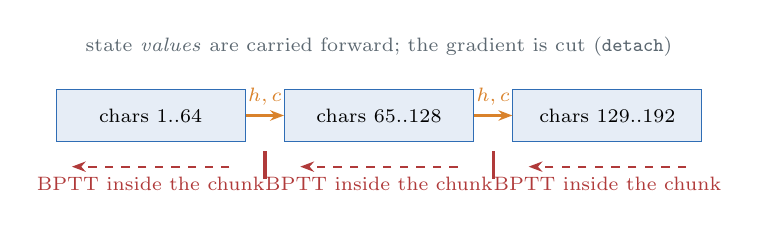
\begin{tikzpicture}[x=10mm,y=7mm,font=\scriptsize]
  \foreach \k/\xx/\lab in {1/0/{chars 1..64},2/2.9/{chars 65..128},3/5.8/{chars 129..192}} {
    \node[draw=cEmb,fill=cEmb!12,minimum width=24mm,minimum height=6.5mm,inner sep=0] (s\k) at (\xx,0) {\lab};
    \draw[flow,draw=cBad,dashed] ([xshift=10mm,yshift=-6.5mm]s\k.center) -- node[below,note,text=cBad]{BPTT inside the chunk} ([xshift=-10mm,yshift=-6.5mm]s\k.center);
  }
  \foreach \a/\b in {1/2,2/3} {
    \draw[flow,draw=cAtt,line width=1pt] (s\a)-- node[above,note,text=cAtt]{$h,c$} (s\b);
    \draw[cBad,line width=1.2pt] ($(s\a.east)!0.5!(s\b.west)+(0,-0.65)$) -- ++(0,-0.5);
  }
  \node[note] at (2.9,1.25) {state \emph{values} are carried forward; the gradient is cut (\texttt{detach})};
\end{tikzpicture}

\vspace{0.5mm}
\raggedright\footnotesize
\key{Truncated BPTT.} A text of a million characters is one sequence; backpropagating through all
of it for each update is unaffordable. Cut it into chunks of $T$ steps: the forward
state crosses chunk borders, gradients stop there. Dependencies longer than $T$ can be
\emph{used} but are not \emph{learned} directly.

\vspace{0.5mm}
\key{Initial state.} $h_0=c_0=0$ at the start of an independent sequence (a window, a document).
Along a stream, each chunk starts from the previous final state (\texttt{stateful=True} in
\texttt{fit}).

\vspace{1mm}
\begin{block}{Gradient clipping by norm \cite{4}}
\footnotesize
$g\;\leftarrow\;g\cdot\min\bigl(1,\ \tau/\|g\|\bigr)$. \ E.g.\ $g=(3,4)$, $\tau=1$: $\|g\|=5$, so
$g\to(0.6,\,0.8)$. Direction kept, length capped at $\tau$; all parameters are scaled together
(\texttt{clip\_grad\_norm\_}).
\end{block}
{\footnotesize \textbf{Honest note}: the divergence on the right needed plain SGD and a large $\eta$.
With Adam we saw gradient spikes but no divergence. We keep $\tau=1$ everywhere as cheap insurance.}
\column{0.47\textwidth}
\centering
\begin{tikzpicture}
\begin{semilogyaxis}[width=8.1cm,height=4.4cm,xmin=0,xmax=400,ymin=0.05,ymax=1e8,
  xlabel={training step},ylabel={gradient norm $\|g\|$ before clipping},label style={font=\scriptsize},
  tick label style={font=\tiny},axis lines=left,ymajorgrids,grid style={cInk!10},ytick={0.1,10,1e3,1e5,1e7},
  legend style={font=\scriptsize,draw=none,fill=none,at={(0.98,0.98)},anchor=north east},legend cell align=left,
  every axis plot/.append style={line width=0.7pt,no marks}]
  \addplot[cBad] table[x=step,y=normoff]{generated/clip.dat}; \addlegendentry{no clipping}
  \addplot[cFfn] table[x=step,y=normon]{generated/clip.dat}; \addlegendentry{clipped at $\tau=0.5$}
\end{semilogyaxis}
\end{tikzpicture}

\vspace{-0.5mm}
\raggedright
{\scriptsize\color{cTok}Measured: simple RNN, $n_h=128$, Shakespeare characters, plain SGD, $\eta=2$, chunks
of 100. Curves and the first two table columns: seed 0.\par}

\vspace{0.5mm}
\footnotesize
{\renewcommand{\arraystretch}{1.15}
\begin{tabular}{@{}lccc@{}}
\toprule
 & largest $\|g\|$ & final loss & diverged\\
\midrule
no clipping & $\clipOffMaxNorm$ & {\color{cBad}\clipOffFinal} & \clipOffDiverged{} of 3\\
clipped, $\tau=0.5$ & $\clipOnMaxNorm$ & \clipOnFinal & \clipOnDiverged{} of 3\\
\bottomrule
\end{tabular}}

\vspace{1mm}
\begin{itemize}
  \item Unclipped, one exploding gradient wrecks the weights: the loss ends \emph{above} the
        \clipUniform{} of a uniform guess. Clipped, the same $\eta$ trains normally.
\end{itemize}
\end{columns}
\end{frame}

% ====================================================================== 13
\begin{frame}{Training II: teacher forcing, unequal lengths, dropout, optimiser}
\begin{columns}[T,onlytextwidth]
\column{0.49\textwidth}
\centering
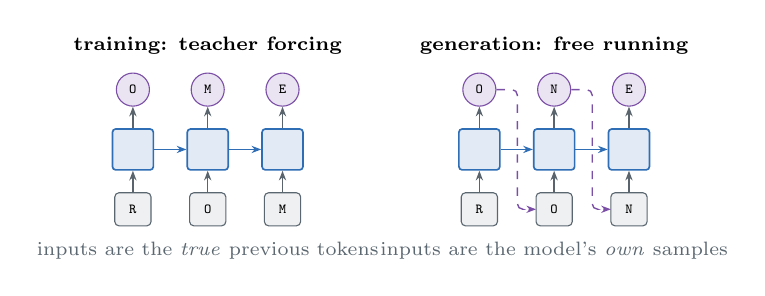
\begin{tikzpicture}[x=9.5mm,y=8mm,font=\scriptsize]
  \begin{scope}
  \foreach \i/\in/\out in {0/R/O,1/O/M,2/M/E} {
    \node[rc] (c\i) at (\i,0) {}; \node[tokbox,minimum width=4.6mm,minimum height=4.2mm,font=\ttfamily\tiny] (x\i) at (\i,-0.95) {\in};
    \node[outp,minimum size=4.2mm,font=\ttfamily\tiny] (y\i) at (\i,0.95) {\out};
    \draw[thin flow] (x\i)--(c\i); \draw[thin flow] (c\i)--(y\i);
  }
  \foreach \i/\j in {0/1,1/2} \draw[thin flow,draw=cEmb] (c\i)--(c\j);
  \node[font=\scriptsize\bfseries] at (1,1.65) {training: teacher forcing};
  \node[note] at (1,-1.6) {inputs are the \emph{true} previous tokens};
  \end{scope}
  \begin{scope}[xshift=44mm]
  \foreach \i/\in/\out in {0/R/O,1/O/N,2/N/E} {
    \node[rc] (c\i) at (\i,0) {}; \node[tokbox,minimum width=4.6mm,minimum height=4.2mm,font=\ttfamily\tiny] (x\i) at (\i,-0.95) {\in};
    \node[outp,minimum size=4.2mm,font=\ttfamily\tiny] (y\i) at (\i,0.95) {\out};
    \draw[thin flow] (x\i)--(c\i); \draw[thin flow] (c\i)--(y\i);
  }
  \foreach \i/\j in {0/1,1/2} { \draw[thin flow,draw=cEmb] (c\i)--(c\j);
    \draw[thin flow,draw=cOut,dashed,rounded corners=2pt] (y\i.east) -- ++(0.28,0) |- ($(x\j.west)+(-0.12,0)$) -- (x\j.west); }
  \node[font=\scriptsize\bfseries] at (1,1.65) {generation: free running};
  \node[note] at (1,-1.6) {inputs are the model's \emph{own} samples};
  \end{scope}
\end{tikzpicture}

\vspace{0.5mm}
\raggedright\footnotesize
\key{Teacher forcing}: in training the input at step $t$ is the true token $y_{t-1}$, whatever the
model predicted. When generating, the model feeds on its own output: an early mistake
(N for M) changes every later input (\emph{exposure bias}; scheduled sampling \cite{13}).

\vspace{0.5mm}
\centering
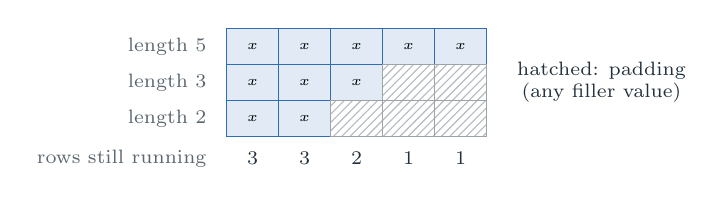
\begin{tikzpicture}[x=6.6mm,y=4.6mm,font=\tiny]
  \foreach \r/\n in {0/5,1/3,2/2} {
    \foreach \i in {1,...,5} {
      \ifnum\i>\n
        \node[draw=cTok!60,pattern=north east lines,pattern color=cTok!45,minimum width=6.6mm,minimum height=4.6mm,inner sep=0] at (\i,-\r) {};
      \else
        \node[draw=cEmb,fill=cEmb!14,minimum width=6.6mm,minimum height=4.6mm,inner sep=0] at (\i,-\r) {$x$};
      \fi
    }
    \node[note,anchor=east] at (0.3,-\r) {length \n};
  }
  \foreach \i/\b in {1/3,2/3,3/2,4/1,5/1} \node[text=cInk,font=\scriptsize] at (\i,-3.1) {\b};
  \node[note,anchor=east] at (0.3,-3.1) {rows still running};
  \node[note,anchor=west,text=cInk] at (5.9,-1) {hatched: padding\\(any filler value)};
\end{tikzpicture}

\raggedright\footnotesize
\key{Unequal lengths}: pad a batch to the longest sequence, then make sure the padding is never
used: \emph{pack} the batch (\texttt{pack\_padded\_sequence}: step $t$ processes only the rows still
running) or mask padded positions out of the loss.
\column{0.48\textwidth}
\small
\begin{block}{Dropout in recurrent networks \cite{14}}
\footnotesize
Apply dropout to the \emph{vertical} connections (input $\to$ layer $\to$ layer $\to$ output), not
to the recurrent connection $h_{t-1}\to h_t$: noise injected into the memory at every step
accumulates and erases it. \texttt{nn.LSTM(dropout=p)} drops between stacked layers only;
\texttt{SeqModel} adds dropout before the output layer.
\end{block}
\begin{block}{Optimiser and learning rate}
\footnotesize
\begin{itemize}
  \item Adam with $\eta$ between $10^{-3}$ and $10^{-2}$ is a robust start for small recurrent
        models. Always clip (slide 12).
  \item \texttt{fit} restores the weights with the lowest validation loss.
\end{itemize}
\end{block}
{\footnotesize
\renewcommand{\arraystretch}{1.15}
\textbf{Settings behind the results} (Adam, clipping at 1)

\vspace{0.5mm}
\begin{tabular}{@{}lccc@{}}
\toprule
 & adding & sunspots & Shakespeare\\
\midrule
hidden size $n_h$ & 32 & 32 & 256\\
sequence / chunk length & 10--80 & 24 & 64\\
batch size & 32 & 64 & 32 streams\\
learning rate & 0.01 & 0.002 & 0.003\\
state between batches & reset & reset & carried\\
\bottomrule
\end{tabular}}
\end{columns}
\end{frame}

% ====================================================================== 14
\begin{frame}{Outputs and losses: forecasting a number, predicting a token}
\begin{columns}[T,onlytextwidth]
\column{0.49\textwidth}
\small
Only the head on top of $h_t$ and the loss depend on the task.
\begin{block}{Regression head (forecasting)}
\footnotesize
$\hat y=w^{\T}h_T+b$: one linear output on the last hidden state. Loss: mean squared error
$\frac1N\sum(\hat y-y)^2$ on standardised values. Report RMSE and MAE in original units
($\hat y\,\sigma+\mu$). For $H$ steps ahead, train one model per horizon (``direct'', used here)
or feed predictions back in (``recursive''; errors accumulate).
\end{block}
\begin{block}{Softmax head (next-token prediction)}
\footnotesize
$z_t=W_y h_t+b_y\in\R^{V}$: the \emph{logits}, one score per vocabulary entry, at every step.
\vspace{-1.5mm}
\[
  p_t=\softmax(z_t),\qquad \mathcal L=-\frac1T\sum_{t=1}^{T}\ln p_t[y_t]\quad\text{(cross-entropy)}
\]
\vspace{-3.5mm}

\key{Perplexity} $=e^{\mathcal L}$: the effective number of equally likely choices per token.
Uniform over $V=\shkVocab$ characters: $\mathcal L=\ln\shkVocab=\shkUniformLoss$, perplexity \shkVocab.

\vspace{0.5mm}
By hand: true tokens got probabilities $(\tfrac12,\tfrac14,\tfrac18,\tfrac12)$.
$\mathcal L=\tfrac14(0.693+1.386+2.079+0.693)=\num{1.213}$, perplexity $\num{3.36}$.
\end{block}
\column{0.48\textwidth}
\centering
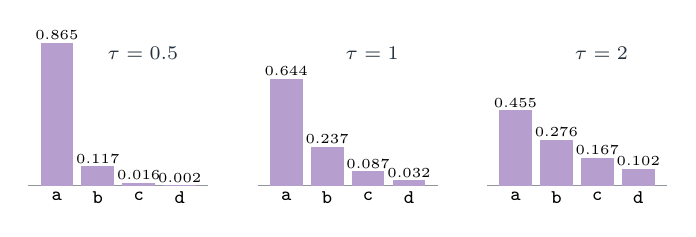
\begin{tikzpicture}[x=5.2mm,y=21mm,font=\tiny]
  \foreach \grp/\xo/\lab/\pa/\pb/\pc/\pd in {0/0/{$\tau=0.5$}/0.865/0.117/0.016/0.002,
        1/5.6/{$\tau=1$}/0.644/0.237/0.087/0.032,2/11.2/{$\tau=2$}/0.455/0.276/0.167/0.102} {
    \draw[cInk!50] (\xo-0.2,0)--(\xo+4.2,0);
    \foreach \p/\k/\ch in {\pa/0/a,\pb/1/b,\pc/2/c,\pd/3/d} {
      \fill[cOut!55] (\xo+\k+0.1,0) rectangle (\xo+\k+0.9,\p);
      \node[anchor=south,inner sep=1pt,font=\fontsize{4.6}{5}\selectfont] at (\xo+\k+0.5,\p) {\p};
      \node[anchor=north,inner sep=2pt,font=\ttfamily\scriptsize] at (\xo+\k+0.5,0) {\ch};
    }
    \node[font=\scriptsize,text=cInk] at (\xo+2.6,0.8) {\lab};
  }
\end{tikzpicture}

\vspace{0.5mm}
{\scriptsize\color{cTok}$\softmax(z/\tau)$ for logits $z=(2,1,0,-1)$ over four tokens a--d.\par}

\vspace{1mm}
\raggedright\small
\begin{block}{Generation: sample, feed back, repeat}
\footnotesize
\begin{enumerate}\setlength{\leftmargini}{1.4em}
  \item Run the prompt through the network; keep the state $(h,c)$.
  \item Sample the next token from $\softmax(z_t/\tau)$.
  \item Feed that token in as the next input: one step, state updated. Go to 2.
\end{enumerate}
\end{block}
\footnotesize
\begin{itemize}
  \item \key{Temperature} $\tau$ rescales the logits before the softmax. $\tau<1$ sharpens the
        distribution (safer, more repetitive); $\tau>1$ flattens it (more varied, more errors);
        $\tau\to0$ is greedy $\arg\max$.
  \item If the true token above is \texttt{b}: loss $=-\ln0.237=\num{1.44}$. Temperature is a
        sampling knob only; the loss is always computed at $\tau=1$.

\end{itemize}
\end{columns}
\end{frame}

% ====================================================================== 15
\begin{frame}[fragile]{Code: the LSTM from scratch, forward and backward (NumPy)}
\vspace{-1mm}
{\footnotesize \texttt{lstm\_numpy.py}: one time step for a batch; \texttt{z} is stacked as [input, forget, candidate, output], the layout of \texttt{torch.nn.LSTM}}
\lstinputlisting[style=py,basicstyle=\ttfamily\fontsize{5.7}{6.8}\selectfont,linerange={27-27,29-39}]{../lstm_numpy.py}
\vspace{0.5mm}
{\footnotesize Backpropagation through time, the loop of \texttt{lstm\_backward}; agrees with finite differences and with PyTorch autograd to $10^{-10}$}
\lstinputlisting[style=py,basicstyle=\ttfamily\fontsize{5.7}{6.8}\selectfont,linerange={65-79}]{../lstm_numpy.py}
\vspace{-0.5mm}
\end{frame}

% ====================================================================== 16
\begin{frame}[fragile]{Code: the training loop and the sampler (PyTorch)}
\vspace{-1mm}
{\footnotesize \texttt{train.py}, inside \texttt{fit()}: one loop for all three tasks (lines verbatim; logging and early stopping omitted)}
\lstinputlisting[style=py,basicstyle=\ttfamily\fontsize{5.7}{6.8}\selectfont,linerange={88-99}]{../train.py}
\vspace{0.5mm}
{\footnotesize \texttt{train.py}, \texttt{generate()}: sampling with temperature; only the state carries the past}
\lstinputlisting[style=py,basicstyle=\ttfamily\fontsize{5.7}{6.8}\selectfont,linerange={200-213}]{../train.py}
\vspace{-0.5mm}
\end{frame}

% ====================================================================== 17
\begin{frame}{Results I: forecasting sunspots, with baselines}
\begin{columns}[T,onlytextwidth]
\column{0.52\textwidth}
\centering
\begin{tikzpicture}
\begin{axis}[width=9.2cm,height=4.6cm,xmin=1948.5,xmax=1984,ymin=0,ymax=290,axis lines=left,
  xlabel={year (test period)},ylabel={monthly sunspot number},label style={font=\scriptsize},
  tick label style={font=\tiny},x tick label style={/pgf/number format/1000 sep=},ymajorgrids,grid style={cInk!10},
  legend columns=3,legend style={font=\scriptsize,draw=none,fill=none,at={(0.5,1.0)},anchor=south,/tikz/every even column/.append style={column sep=2mm}},
  legend cell align=left,every axis plot/.append style={no marks}]
  \addplot[cInk!55,line width=0.5pt] table[x=year,y=true]{generated/forecast.dat}; \addlegendentry{observed}
  \addplot[cAtt,line width=0.9pt] table[x=year,y=lstm]{generated/forecast.dat}; \addlegendentry{LSTM}
  \addplot[cFfn,line width=0.9pt,densely dashed] table[x=year,y=linear]{generated/forecast.dat}; \addlegendentry{linear AR}
\end{axis}
\end{tikzpicture}

\vspace{-0.5mm}
\raggedright
{\scriptsize\color{cTok}6-month-ahead forecasts on the \sunNtest{} test months, each made from the 24 months
before it. LSTM: seed 0. The test period holds the largest cycle on record (peak \sunTestMax; training
maximum \sunTrainMax), so every model must extrapolate.\par}

\vspace{0.5mm}
\raggedright\footnotesize
\textbf{Setup} (\texttt{python train.py -{}-task sunspots [-{}-horizon 6]}): window of 24 months $\to$
LSTM, $n_h=32$, \sunParams{} parameters $\to$ linear head on $h_{24}$. Chronological 70/15/15 split,
scaling from 1749--\sunTrainEnd.

\vspace{0.5mm}
\textbf{Baselines.} \key{Persistence}: the last observed value. \key{Seasonal-naive}: the value
132 months earlier (the mean solar cycle is about 11 years). \key{Linear AR}: least-squares linear
map from the same 24 values, 25 parameters.
\column{0.45\textwidth}
\footnotesize
{\renewcommand{\arraystretch}{1.1}
\begin{tabular}{@{}lcccc@{}}
\toprule
 & \multicolumn{2}{c}{1 month ahead} & \multicolumn{2}{c}{6 months ahead}\\
test set & RMSE & MAE & RMSE & MAE\\
\midrule
persistence & \sunPersistRmseOne & \sunPersistMaeOne & \sunPersistRmseSix & \sunPersistMaeSix\\
seasonal-naive & \sunSeasonalRmseOne & \sunSeasonalMaeOne & \sunSeasonalRmseSix & \sunSeasonalMaeSix\\
linear AR(24) & \textbf{\sunLinearRmseOne} & \sunLinearMaeOne & \textbf{\sunLinearRmseSix} & \sunLinearMaeSix\\
\midrule
simple RNN & \sunRnnRmseOne{\tiny$\pm$\sunRnnRmseStdOne} & \sunRnnMaeOne & \sunRnnRmseSix{\tiny$\pm$\sunRnnRmseStdSix} & \sunRnnMaeSix\\
GRU & \sunGruRmseOne{\tiny$\pm$\sunGruRmseStdOne} & \sunGruMaeOne & \sunGruRmseSix{\tiny$\pm$\sunGruRmseStdSix} & \sunGruMaeSix\\
LSTM & \sunLstmRmseOne{\tiny$\pm$\sunLstmRmseStdOne} & \sunLstmMaeOne & \sunLstmRmseSix{\tiny$\pm$\sunLstmRmseStdSix} & \sunLstmMaeSix\\
\bottomrule
\end{tabular}}

\vspace{0.5mm}
{\scriptsize\color{cTok}Sunspot-number units. Recurrent models: mean $\pm$ std over 3 seeds.\par}

\vspace{0.5mm}
\begin{block}{Honest reading}
\footnotesize
\begin{itemize}
  \item Every learned model beats persistence and seasonal-naive.
  \item \textbf{The LSTM does not beat the 25-parameter linear model}: its RMSE is below linear
        AR in \sunLstmWinsOne{} of 3 seeds at 1 month and \sunLstmWinsSix{} of 3 at 6 months.
        Linear baselines are hard to beat on such series \cite{19}.
  \item RNN, GRU and LSTM are within noise of each other: a 24-step window holds no
        long-range dependency for gates to protect.
\end{itemize}
\end{block}

\end{columns}
\end{frame}

% ====================================================================== 18
\begin{frame}[fragile]{Results II: a character-level language model on Tiny Shakespeare}
\begin{columns}[T,onlytextwidth]
\column{0.44\textwidth}
\centering
\begin{tikzpicture}
\begin{axis}[width=7.9cm,height=4.3cm,xmin=0,xmax=\shkSteps,ymin=1.2,ymax=3.5,axis lines=left,
  xlabel={training step},ylabel={loss (nats per character)},label style={font=\scriptsize},
  tick label style={font=\tiny},ymajorgrids,grid style={cInk!10},
  legend style={font=\scriptsize,draw=none,fill=none,at={(0.98,0.98)},anchor=north east},legend cell align=left,
  every axis plot/.append style={line width=1.1pt,mark size=1.2pt}]
  \addplot[cEmb,mark=*] table[x=step,y=train]{generated/shk_curve.dat}; \addlegendentry{training}
  \addplot[cAtt,mark=square*] table[x=step,y=val]{generated/shk_curve.dat}; \addlegendentry{validation}
  \addplot[cTok,dashed,no marks,domain=0:\shkSteps,samples=2] {\shkBigramLoss}; \addlegendentry{bigram counts (test)}
\end{axis}
\end{tikzpicture}

\vspace{0.5mm}
{\footnotesize
\renewcommand{\arraystretch}{1.15}
\begin{tabular}{@{}lccc@{}}
\toprule
test set (\shkNtest{} chars) & loss & perplexity & bits/char\\
\midrule
uniform over \shkVocab{} & \shkUniformLoss & \shkUniformPpl & --\\
unigram counts & \shkUnigramLoss & \shkUnigramPpl & --\\
bigram counts & \shkBigramLoss & \shkBigramPpl & --\\
\textbf{LSTM} & \textbf{\shkTestLoss} & \textbf{\shkTestPpl} & \shkTestBits\\
\bottomrule
\end{tabular}}

\vspace{1mm}
\raggedright
{\scriptsize\color{cTok}\texttt{python train.py -{}-task shakespeare}: embedding 32 $\to$ LSTM, $n_h=256$ $\to$
softmax over \shkVocab; \shkParams{} parameters. \shkSteps{} steps of truncated BPTT (32 streams $\times$ 64
characters, \shkEpochs{} passes over \shkNtrain{} training characters), \shkSeconds{} s on one CPU
core. Split by position: 90\% train, 5\% validation, 5\% test. One run. Each training point is the
mean over the preceding 250 steps.\par}
\column{0.54\textwidth}
\footnotesize
\textbf{LSTM sample, temperature 0.5} \ (prompt \texttt{ROMEO:})
\lstinputlisting[style=txt]{generated/sample_05.txt}
\textbf{LSTM sample, temperature 1.0}
\lstinputlisting[style=txt]{generated/sample_10.txt}
\textbf{Bigram baseline sample} \ (one character of context; / marks a line break)
\lstinputlisting[style=txt]{generated/sample_bigram.txt}
\vspace{0.5mm}
\begin{itemize}
  \item The bigram table sees one character of context: perplexity \shkBigramPpl. The
        LSTM carries context in its state and reaches \shkTestPpl: it has learned spelling, line
        lengths and the speaker-name layout.
  \item $\tau=0.5$ gives mostly real words; $\tau=1$ samples the model's own distribution and
        shows its errors.
  \item Validation loss is still falling: a two-minute CPU run, not a converged model.
\end{itemize}
\end{columns}
\end{frame}

% ====================================================================== 19
\begin{frame}{Where LSTMs stand today, relative to transformers}
\begin{columns}[T,onlytextwidth]
\column{0.50\textwidth}
\centering
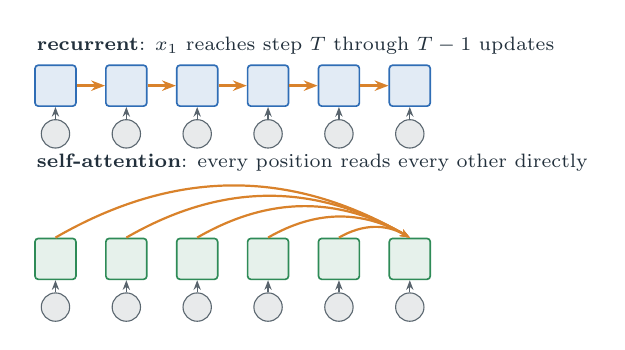
\begin{tikzpicture}[x=9mm,y=6.8mm,font=\scriptsize]
  \begin{scope}
  \foreach \i in {0,...,5} { \node[rc] (c\i) at (\i,0) {}; \node[inp] (x\i) at (\i,-0.9) {}; \draw[thin flow] (x\i)--(c\i); }
  \foreach \i/\j in {0/1,1/2,2/3,3/4,4/5} \draw[flow,draw=cAtt,line width=1pt] (c\i)--(c\j);
  \node[note,text=cInk,anchor=west] at (-0.4,0.75) {\textbf{recurrent}: $x_1$ reaches step $T$ through $T-1$ updates};
  \end{scope}
  \begin{scope}[yshift=-22mm]
  \foreach \i in {0,...,5} { \node[rc,draw=cFfn,fill=cFfn!12] (c\i) at (\i,0) {}; \node[inp] (x\i) at (\i,-0.9) {}; \draw[thin flow] (x\i)--(c\i); }
  \foreach \i in {0,...,4} \draw[thin flow,draw=cAtt,line width=0.8pt] (c\i.north) to[bend left=30] (c5.north);
  \node[note,text=cInk,anchor=west] at (-0.4,1.8) {\textbf{self-attention}: every position reads every other directly};
  \end{scope}
\end{tikzpicture}

\vspace{1mm}
{\footnotesize
\renewcommand{\arraystretch}{1.05}
\begin{tabular}{@{}lcc@{}}
\toprule
per layer, length $T$, width $d$ & recurrent & self-attention\\
\midrule
computation & $O(T\,d^2)$ & $O(T^2 d)$\\
sequential operations & $O(T)$ & $O(1)$\\
path length between two positions & $O(T)$ & $O(1)$\\
memory while generating & $O(d)$ state & $O(T\,d)$ cache\\
\bottomrule
\end{tabular}

{\scriptsize\color{cTok}First three rows: Table 1 of \cite{17}.\par}}

\vspace{1mm}
\raggedright\footnotesize
\textbf{Why transformers took over} (2017 on): all positions of a training sequence are
processed in parallel, and any two are one step apart: no long chain of Jacobians.

\vspace{0.5mm}
\textbf{Rule of thumb}: lots of data and offline training, use a transformer. Little data,
a latency budget or a live stream: try a GRU or LSTM, and a linear baseline first.
\column{0.47\textwidth}
\small
\begin{block}{Where recurrent models are still a sound choice}
\footnotesize
\begin{itemize}
  \item \textbf{Streaming and low latency}: one input in, one output out, constant memory and
        cost per step, no context window to manage. On-device speech, sensor monitoring, control.
  \item \textbf{Small data}: a 5k-parameter LSTM trains in seconds on a CPU (slides 11, 17).
  \item \textbf{Time series}: attention shows no clear win; simple linear models have matched or
        beaten transformer forecasters \cite{19}, as the linear AR did here.
\end{itemize}
\end{block}
\begin{block}{The ideas outlived the architecture}
\footnotesize
\begin{itemize}
  \item The additive path of the cell state reappears as the residual connection in every
        transformer block.
  \item Recurrence is being revisited: xLSTM \cite{18} changes the gating and memory of the LSTM
        and reports results competitive with transformers on language modelling. Independent
        large-scale confirmation is still limited.
\end{itemize}
\end{block}

\end{columns}
\end{frame}

% ====================================================================== 20
\begin{frame}{References and how to run the code}
\fontsize{6.4}{7.9}\selectfont
\begin{columns}[T,onlytextwidth]
\column{0.49\textwidth}
\begin{enumerate}[{[1]}]\setlength{\itemsep}{0.6pt}
\item Elman. \emph{Finding Structure in Time.} Cognitive Science 14(2), 1990.
\item Werbos. \emph{Backpropagation Through Time: What It Does and How to Do It.} Proceedings of the IEEE 78(10), 1990.
\item Bengio, Simard, Frasconi. \emph{Learning Long-Term Dependencies with Gradient Descent is Difficult.} IEEE Transactions on Neural Networks 5(2), 1994.
\item Pascanu, Mikolov, Bengio. \emph{On the Difficulty of Training Recurrent Neural Networks.} ICML 2013. arXiv:1211.5063
\item Hochreiter, Schmidhuber. \emph{Long Short-Term Memory.} Neural Computation 9(8), 1997.
\item Gers, Schmidhuber, Cummins. \emph{Learning to Forget: Continual Prediction with LSTM.} Neural Computation 12(10), 2000.
\item Greff, Srivastava, Koutn\'ik, Steunebrink, Schmidhuber. \emph{LSTM: A Search Space Odyssey.} IEEE TNNLS 28(10), 2017. arXiv:1503.04069
\item Jozefowicz, Zaremba, Sutskever. \emph{An Empirical Exploration of Recurrent Network Architectures.} ICML 2015.
\item Cho, van Merri\"enboer, Gulcehre, Bahdanau, Bougares, Schwenk, Bengio. \emph{Learning Phrase Representations using RNN Encoder--Decoder for Statistical Machine Translation.} EMNLP 2014. arXiv:1406.1078
\item Chung, Gulcehre, Cho, Bengio. \emph{Empirical Evaluation of Gated Recurrent Neural Networks on Sequence Modeling.} 2014. arXiv:1412.3555
\item Schuster, Paliwal. \emph{Bidirectional Recurrent Neural Networks.} IEEE Transactions on Signal Processing 45(11), 1997.
\item Sutskever, Vinyals, Le. \emph{Sequence to Sequence Learning with Neural Networks.} NeurIPS 2014. arXiv:1409.3215
\end{enumerate}
\column{0.49\textwidth}
\begin{enumerate}[{[1]}]\setlength{\itemsep}{0.6pt}
\setcounter{enumi}{12}
\item Bengio, Vinyals, Jaitly, Shazeer. \emph{Scheduled Sampling for Sequence Prediction with Recurrent Neural Networks.} NeurIPS 2015. arXiv:1506.03099
\item Zaremba, Sutskever, Vinyals. \emph{Recurrent Neural Network Regularization.} 2014. arXiv:1409.2329
\item Graves. \emph{Generating Sequences With Recurrent Neural Networks.} 2013. arXiv:1308.0850
\item Karpathy, Johnson, Fei-Fei. \emph{Visualizing and Understanding Recurrent Networks.} 2015. arXiv:1506.02078
\item Vaswani, Shazeer, Parmar, Uszkoreit, Jones, Gomez, Kaiser, Polosukhin. \emph{Attention Is All You Need.} NeurIPS 2017. arXiv:1706.03762
\item Beck, P\"oppel, Spanring, Auer, Prudnikova, Kopp, Klambauer, Brandstetter, Hochreiter. \emph{xLSTM: Extended Long Short-Term Memory.} 2024. arXiv:2405.04517
\item Zeng, Chen, Zhang, Xu. \emph{Are Transformers Effective for Time Series Forecasting?} AAAI 2023. arXiv:2205.13504
\end{enumerate}
\vspace{0.3mm}
{\color{cInk}\textbf{Data.} Monthly sunspot numbers 1749--1983 (\texttt{jbrownlee/Datasets} on GitHub).
Tiny Shakespeare (\texttt{karpathy/char-rnn}; character models as in \cite{15,16}).}

\vspace{0.5mm}
{\fontsize{6.6}{8.1}\selectfont\color{cInk}
\textbf{Run it} with \texttt{python <file>} (NumPy, PyTorch; CPU only)

\vspace{0.5mm}
\begin{tabular}{@{}l@{\ \ }l@{}}
\texttt{test\_lstm.py} & eight checks, incl.\ BPTT vs.\ finite differences\\
\texttt{walkthrough.py} & hand calculations (slides 3--5, 7, 8, 10, 12--14)\\
\texttt{lstm\_numpy.py} & NumPy LSTM vs.\ \texttt{torch.nn.LSTM}\\
\texttt{train.py -{}-task sunspots} & or \texttt{adding}, \texttt{shakespeare}; see \texttt{-{}-help}\\
\texttt{experiments.py} & figures for slides 3, 8--12, 17, 18\\
\end{tabular}

\vspace{0.5mm}
\textbf{Exercises.} Train with \texttt{-{}-forget\_bias 0}. Swap \texttt{-{}-model gru} into the character model.}
\end{columns}
\end{frame}

\end{document}
